% Tento soubor nahraďte vlastním souborem s obsahem práce.
%=========================================================================
% Autoři: Michal Bidlo, Bohuslav Křena, Jaroslav Dytrych, Petr Veigend a Adam Herout 2019

% Pro kompilaci po částech (viz projekt.tex), nutno odkomentovat a upravit
%\documentclass[../projekt.tex]{subfiles}
%\begin{document}
\chapter{Úvod}
Problém obchodního cestujícího je obtížný diskrétní optimalizační problém, a pro více míst je v rozumném čase neřešitelný, pokud by se procházely všechny možnosti. V kapitole 2 popíši problém obchodního cestujícího. V kapitole 3 se seznámíme s algoritmy a heuristikami, které se využívají k řešení tohoto problému. Asi nejúspěšnější z nich je \textbf{Lin-Kernighan heuristic}. V kapitole 4 popíši základní teorii algoritmů, které jsem si vybral. Jedním z nich je \textbf{ACO}, a druhým je \textbf{MyAlgo}. V kapitole 5 se zaměřím na konkrétní implementaci těchto dvou algoritmů. V kapitole 6 se zaměřím na program jako celek s všemi pomocnými soubory. V kapitole 7 jsou popsány funkce uživatelského rozhraní, jako je například import míst z mapy nebo popsané jednotlivé funkce widgetů. V kapitole 8 se zaměřím na implementaci ACO a MyAlgo. Oba algoritmy budou testovány až do 1500 míst, a od 1500 míst se zaměřím pouze na MyAlgo. Testy jsem prováděl až do 22775 míst.





\chapter{Problém obchodního cestujícího}
Problém byl poprvé matematicky formulován v 19. století dvěma matematiky, z nichž jeden byl Sir William Rowam Hamilton a druhý Thomas Penyngton Kirkman. Nicméně předpokládá se, že obecnou podobu TSP poprvé studoval Karl Menger. Slovní definice problému může znít následovně: Je dána množina měst, neboli míst. Pro přesun z jednoho místa do druhého je třeba využít cestu, která má určitou vzdálenost. Každé místo má cestu ke všem ostatním místům. Podstatou problému je najít nejlepší možný způsob, jak navštívit všechna místa a vrátit se do výchozího místa, a to minimalizací cestovních nákladů nebo cestovní vzdálenosti. Matematicky to můžeme vyjádřit tak, že hledáme v ohodnoceném úplném grafu nejkratší hamiltonovskou kružnici. S rostoucím počtem míst roste počet potenciálních řešení, které je třeba prohledat. Celkový počet možných tras pokrývajících všechna města, která je třeba navštívit (lze je zapsat jako množinu proveditelných řešení TSP), roste s počtem měst n a je dán jako:
\begin{center}
    \scalebox{1.5}{$ O = \frac{(n-1)!}{2} $}
\end{center}
Například pro 20 míst máme zhruba $1.2 * 10^{18}$ tras, které mohou být potenciálně optimálním řešením, a to je pouze pro 20 míst. Pro tak velký počet potenciálních řešení je nemožné prohledat všechny trasy v rozumném čase, i pro superpočítače. Proto se při řešení problému používají algoritmy, které neprohledávají všechny trasy, ale pouze ty více "atraktivní" pro algoritmus. Tyto algoritmy mohou skončit po určitém počtu iterací nebo po splnění nějaké podmínky, například 3-opt, když se řešení nezlepší. Tuto informaci jsem převzal z \cite{TSPbook}.




\chapter{Přehled algoritmů pro řešení problému obchodního cestujícího}
\section{Nearest Neighbor Algorithm}
Jde asi o nejjednodušší algoritmus pro řešení problému obchodního cestujícího. Časová složitost algoritmu je $O(n^2)$. Algoritmus by mohl vypadat následovně: Vytvořím si datovou strukturu, která bude ukládat navštívená místa. Zvolím si místo, ve kterém budu začínat, například náhodně. Uložím ho jako aktuální místo, ve kterém jsem, a vložím ho do struktury navštívených míst. Zvolím cestu do následujícího místa takovou, která je nejkratší možná a zároveň se místo, kam cesta vede, nenachází v navštívených místech. Následující místo zvolím jako aktuální a vložím jej do struktury pro navštívená místa. To opakuji, dokud nenavštívím všechna místa.
\section{Greedy Algorithm}
Je  to jednoduchý algoritmus, který se používá v různých oblastech, jako je například optimalizace a teorie grafů. Jeho princip spočívá v tom, že v každém kroku algoritmu se vybere nejlepší (nebo nejhorší) možnost na základě aktuální situace a nevrací se zpět, aby se nějaká dřívější volba změnila. Tento postup může vést k rychlému a jednoduchému řešení problému, ale v některých případech může být neefektivní a vést k špatnému výsledku.

Jedním z příkladů použití Greedy algoritmu může být problém hledání nejkratší cesty v grafu. Algoritmus by se mohl rozhodnout v každém kroku pro hranu s nejmenší váhou a pokračovat tímto způsobem, dokud není nalezena cesta mezi dvěma uzly. Tento postup ale nemusí vést k nejkratší cestě. Dalším příkladem aplikace algoritmu může být problém obchodního cestujícího, kdy se postupně volí nejkratší cesty, které lze spojit a postupně spojují místa, dokud nejsou navštívena všechna místa.
\section{2-opt}
Algoritmus 2-opt je speciálním případem algoritmu $\lambda$-opt, kde v každém kroku jsou nahrazeny $\lambda$ odkazy aktuální trasy novými $\lambda$ odkazy takovým způsobem, aby byla dosažena kratší trasa. Jinými slovy, v každém kroku se dosáhne kratší trasy tím, že jsou odstraněny $\lambda$ odkazy a výsledné cesty jsou spojeny novým způsobem, případně některé z nich jsou obráceny.
Algoritmus $\lambda$-opt je založen na konceptu $\lambda$-optimality:
Trasa je označena jako $\lambda$-optimální (nebo jednoduše $\lambda$-opt), pokud není možné dosáhnout kratší trasy nahrazením jakýchkoli $\lambda$ odkazů jinou sadou $\lambda$ odkazů \cite{helsgaun2000effective}. Praktické využití je popsáno v \ref{sec:NNA 3opt in ACO}.

\section{Genetic Algorithm}
Genetický algoritmus je metoda pro řešení omezených i neomezených optimalizačních problémů, která je založena na přírodním výběru, procesu, který řídí biologickou evoluci. Genetický algoritmus opakovaně modifikuje populaci individuálních řešení. V každém kroku genetický algoritmus vybírá jedince z aktuální populace, kteří se stanou rodiči a používá je k vytvoření potomků pro další generaci. V průběhu následujících generací se populace "vyvíjí" směrem k optimálnímu řešení. Genetický algoritmus lze aplikovat k řešení různých optimalizačních problémů, které nejsou dobře vhodné pro standardní optimalizační algoritmy, včetně problémů, ve kterých je cílová funkce nespojitá, nediferencovatelná, stochastická nebo silně nelineární. Genetický algoritmus může řešit problémy kombinovaného celočíselného programování, kde jsou některé komponenty omezeny být celočíselné. \cite{mathworks-genetic-algorithm}
\section{Lin-Kernighan Heuristic}
Jedná se asi o nejlepší algoritmus pro řešení problému obchodního cestujícího. Poprvé byl publikován v roce 1973 v \cite{LinKernighan1973}. Existují různé varianty a vylepšení tohoto algoritmu, které jsou velmi efektivní i při velkém počtu měst. Jak je zmíněno v \cite{helsgaun2000effective}, celková implementace a návrh algoritmu jsou velmi složité. Algoritmus Lin-Kernighan je úzce spjat s algoritmem $\lambda$-opt.

Algoritmus Lin-Kernighan patří do třídy tzv. lokálních optimalizačních algoritmů. Je specifikován pomocí výměn (nebo tahů), které umožňují převést jednu trasu na jinou. Po získání proveditelné trasy algoritmus opakovaně provádí výměny, které snižují délku aktuální trasy, dokud není dosaženo trasy, pro kterou žádná výměna neposkytuje vylepšení. Tento proces může být opakován mnohokrát z různých počátečních tras generovaných nějakým náhodným způsobem.

 











\section{Ant Colony Optimization Algorithm (ACO)} 
Mravenci projevují složité sociální chování, které již dlouho přitahuje pozornost lidí. Pravděpodobně jedním z nejzřetelnějších chování, které můžeme pozorovat, je tvorba takzvaných mravenišť. Když jsme byli mladí, mnozí z nás možná šlápli na takovou mravenčí dálnici nebo překážku na její cestě jen proto, abychom viděli, jak mravenci na takové rušení zareagují. Možná jsme se také ptali, kam tato mraveniště vedou nebo jak vůbec vznikají. Pro většinu z nás se takové otázky mohou stát méně naléhavými, jakmile dospějeme a začneme studovat jiné předměty, jako jsou počítačové vědy, matematika a podobně. Nicméně existuje značný počet výzkumníků, hlavně biologů, kteří studují chování mravenců detailně.

Jedním z nejzajímavějších chování, které mravenci projevují, je schopnost určitých druhů mravenců najít to, co počítačoví vědci nazývají nejkratšími cestami. Biologové experimentálně prokázali, že toto je možné díky využití komunikace založené pouze na feromonech, pachové chemické látky, kterou mravenci mohou ukládat a cítit. Právě toto chování inspirovalo počítačové vědce k vývoji algoritmů pro řešení optimalizačních problémů. První pokusy v této oblasti se objevily v 90. letech a mohou být považovány za spíše "hrací" ukázky, i když důležité pro naznačení obecné platnosti přístupu. Od té doby tyto a podobné myšlenky přitahují stále větší množství výzkumu a optimalizace mravenčí kolonií (ACO) je jedním z výsledků těchto úsilí. Ve skutečnosti jsou ACO algoritmy nejúspěšnější a nejuznávanější algoritmické techniky založené na mravenčím chování. 
Kolonie mravenců a obecně společnosti sociálních hmyzu jsou distribuované systémy, které navzdory jednoduchosti svých jednotlivců prezentují vysoce strukturovanou sociální organizaci. Díky této organizaci mohou kolonie mravenců dokázat složité úkoly, které v některých případech dalece převyšují individuální schopnosti jednoho mravence.

Obor algoritmů mravenců zkoumá modely odvozené z pozorování skutečného chování mravenců a používá tyto modely jako zdroj inspirace pro návrh nových algoritmů pro řešení optimalizačních a distribuovaných řídicích problémů. Hlavní myšlenkou je, že samoorganizační principy, které umožňují vysoce koordinované chování skutečných mravenců, lze využít k souřadění populací umělých agentů, kteří spolupracují na řešení výpočetních problémů.

Několik různých aspektů chování kolonií mravenců inspirovalo různé druhy algoritmů mravenců. Příklady jsou hledání potravy, rozdělení práce, třídění potomstva a kooperativní přeprava. V těchto případech koordinují mravenci své aktivity prostřednictvím stigmergie, formy nepřímé komunikace prostřednictvím modifikací prostředí. Biologové ukázali, že mnoho chování na úrovni kolonie pozorovaných u sociálního hmyzu lze vysvětlit poměrně jednoduchými modely, ve kterých je přítomna pouze stigmergická komunikace. Jinými slovy, biologové ukázali, že často stačí zvážit stigmergickou, nepřímou komunikaci k vysvětlení toho, jak mohou sociální hmyz dosáhnout samoorganizace. Myšlenkou za algoritmy mravenců je tedy využít formu umělé stigmergie k souřadění společností umělých agentů.
Jedním z nejlepších příkladů algoritmů mravenců je známý jako optimalizace kolonií mravenců nebo ACO, který se zaměřuje na diskrétní optimalizační problémy \cite{Colony2004}.
\subsection{Rozdíly skutečných a simulovaných mravenců}
\begin{itemize}
\item{ Umělí mravenci jsou vytvořeni tak, aby spolupracovali a využívali informace, které zanechávají ostatní mravenci. Ve skutečnosti se jednotliví mravenci snaží získat co nejvíce potravy pro sebe.}


\item{V ACO algoritmu jsou feromony inicializovány na nulovou hodnotu, zatímco v přírodě mravenci používají feromony, které už byly zanechány jinými mravenci.}
\item{ Skuteční mravenci vypouští feromon neustále, umělí mravenci značkují cestu 
„feromonem“ pouze při návratu do mraveniště. \cite{zbřil2012zaklady}}

\item{Umělí mravenci mají tendenci procházet kratší cestami, zatímco v přírodě mohou být cesty dlouhé, ale mohou obsahovat více potravy.}

\item{Umělí mravenci v ACO algoritmu se vypořádávají s problémy s paralelizací a koordinací, které nejsou relevantní pro skutečné mravence.}
\end{itemize}

\subsection{Popis algoritmu}
ACO je metaheuristický algoritmus inspirovaný chováním mravenců. Jeho principem je vytvoření umělého mraveniště, které obsahuje počáteční řešení optimalizačního problému, a postupné procházení řešení umělými mravenci. Mravenci vytvářejí feromonové stopy, které informují ostatní mravence o kvalitě cesty, kterou prošli. Tímto způsobem mravenci postupně hledají nejlepší cestu řešení daného problému.
Princip algoritmu spočívá v iterativním procházení umělého mraveniště několikrát za sebou, přičemž v každé iteraci se aktualizují feromonové stopy a vybírají se nejlepší cesty. Výsledkem algoritmu je nejlepší nalezené řešení daného problému.
Algoritmus se využívá k řešení optimalizačních problémů v různých oblastech, jako je například logistika, plánování dopravy nebo hledání nejlepších tras v sítích.

\subsection{Aplikace algoritmu na problém obchodního cestujícího}

\begin{enumerate}
\item Nastaví se počáteční stav intenzit feromonů na $\tau_{ij} = \alpha$. $\alpha$ by mělo být kladné číslo blízké 0, obvykle v rozmezí (0.01,0.5), pro všechny cesty mezi místy $i$ a $j$ kde $(i = 1...N,j = 1...N, i \neq j, N$ je celkový počet míst).
\item Dále se vytvoří zvolený počet mravenců.
\item V každém mravenci se začne iterovat přes $y = (0...Y-1)$, kde $Y$ je počet iterací, který jste nastavili.
\item V každé iteraci v rámci jednoho mravence se vybere počáteční místo.
\item Následně v každé iteraci v rámci mravence se vybírá každé další místo, které mravenec ještě nenavštívil na základě vztahu:
\begin{equation*}
p_{ij}=\frac{\left[\tau_{ij}\right]^\alpha\left[\eta_{ij}\right]^\beta}{\sum_{l=1}^{N}\left[\tau_{il}\right]^\alpha\left[\eta_{il}\right]^\beta}
\end{equation*}
kde $p_{ij}$ je pravděpodobnost cesty z místa $i$ do místa $j$, $\eta_{ij} = 1/d_{ij}$ a $\alpha$ a $\beta$ jsou empirické konstanty. Pravděpodobnost cesty $p_{ij}$ se vypočítá pro každé nenavštívené místo z aktuálního místa. Na základě těchto pravděpodobností se rozhodne, které místo bude další. Tento proces se opakuje, dokud mravenec nenavštíví všechna místa v rámci jedné iterace. Poté se v každé iteraci aktualizují feromony. Pro tento účel se nejprve uzamkne zámek, protože feromony jsou sdílené pro každého mravence. $\Delta \tau$ představuje přírůstek feromonů na všech cestách, které mravenec navštívil v rámci jedné iterace:

\begin{equation*}
\scalebox{1.5}{$\Delta \tau = \frac{Q}{L}$}
\end{equation*}

Q je zvolená konstanta, která určuje, kolik feromonů mravenec vyloučí během jedné iterace. L je délka cesty.

Následně se v každé iteraci v rámci vlákna aplikuje postupné vyprchávání feromonů na všechny cesty, nikoliv pouze na ty, které mravenec v rámci iterace navštívil.

\begin{equation*}
    \scalebox{1.5}{$\tau = \tau*(1-\rho) $}
\end{equation*}

\item Dále se porovná, zda právě dokončená cesta není nejlepší možná. Zde je také potřeba použít zámek. Pokud je cesta lepší než všechny ostatní cesty v rámci všech mravenců, uloží se tato cesta. Tento proces probíhá v každé iteraci v rámci každého vlákna.
\item Nakonec se v rámci mravence inkrementuje čítač y a vrátí se na bod 3.

\end{enumerate}



\subsection{Mnou modifikovaný algoritmus s využitím dalších algoritmů}
Jsou zde tři hlavní rozdíly: větší využití Q0 v bodě 1, použití dvou dalších algoritmů (Nearest Neighbor Algorithm) pro nastavení počátečních feromonů a více využití 2-opt k přeskupování cest, aby vzniklo lepší řešení (viz sekce \ref{sec:NNA 3opt in ACO}).

\begin{enumerate}
\item Nastaví se počáteční stav intenzity feromonů na $\tau_{ij} = \alpha$, kde $\alpha$ by mělo být kladné číslo blízké nule, obvykle v rozmezí (0,01 až 0,5). To se provede pro všechny cesty mezi místy $i$ a $j$, kde $(i = 1...N, j = 1...N, i \neq j)$ a $N$ je celkový počet míst.
\item Začne se iterovat přes $z = (0...Z-1)$, kde $Z$ je počet iterací, kolikrát se má použít Nearest Neighbor Algorithm.
\item V rámci iterace se zvolí počáteční místo $m$, které ještě nebylo v žádné iteraci zvoleno.
\item Použije se v rámci iterace Nearest Neighbor Algorithm, ale pouze pro omezený počet míst $F$, který je obvykle nastaven na 2 až 4 místa.
\item V rámci iterace se inkrementuje $\tau_{ij}$ na cestách, které byly v rámci Nearest Neighbor Algorithm použity, pomocí vztahu:
\begin{equation*}
\scalebox{1.5}{$\Delta \tau = \frac{Q}{L}$}
\end{equation*}
Konstanta Q je zvolena jako množství feromonů, které mravenec vyloučí. Konstanta L reprezentuje délku cesty.
\item Inkrementuje se čítač z a program se vrací na bod 2.
\item Následně se vytvoří požadovaný počet mravenců (agentů), které reprezentují v mé implementaci vlákna.
\item V každém vláknu se iteruje přes y = (0...Y-1), kde Y je počet iterací, který byl nastaven.
\item V každé iteraci v rámci vlákna se vybere počáteční místo.
\item Poté se v každé iteraci v rámci vlákna vybírá každé další místo, které mravenec ještě nenavštívil na základě vztahu:
\begin{center}
\begin{equation*}
\scalebox{1.5}{$p_{i j}=\frac{\left[\tau_{i j}\right]^\alpha\left[\eta_{i j}\right]^\beta}{\sum_{1}^{N}\left[\tau_{i l}\right]^\alpha\left[\eta_{i l}\right]^\beta}$}
\end{equation*}
\end{center}
kde $p_{i j}$ je pravděpodobnost cesty z místa i do místa j a $\eta_{i j} = 1/d_{i j}$. Pravděpodobnost cesty $p_{i j}$ se vypočítá pro každé nenavštívené místo z aktuální pozice. Dle pravděpodobností se rozhodne, které místo bude následující. Toto se opakuje, dokud mravenec (vlákno) v rámci jedné iterace nenavštíví všechna místa.
\item V algoritmu figuruje také volba na základě konstanty Q0. Pokud pseudonáhodně vygenerované číslo v rozmezí (0,1) je menší než konstanta Q0, zvolí se cesta s největší pravděpodobností, tj. "nejvýhodnější".


\item Poté v každé iteraci v rámci vlákna se aktualizují feromony, aby k tomu mohlo dojít je nejprve zamknout zámek, jelikož jsou feromony pro každého mravence sdílené. $\Delta \tau$ je přírůstek feromonů na všech cestách, které mravenec v rámci jedné iterace navštívil. 
\begin{equation*}
    \scalebox{1.5}{$\Delta \tau = \frac{Q}{L} $}
\end{equation*}

Q je zvolená konstanta kolik mravenec vyloučí feromonů za jednu iteraci. L je délka cesty. 
\item V každé iteraci v rámci vlákna se aplikuje i postupné vyprchávání feromonů a to již pro všechny cesty ne pouze ty, které mravenec v rámci iterace navštívil. 
\begin{equation*}
    \scalebox{1.5}{$\tau = \tau*(1-\rho) $}
\end{equation*}

\item Dále se porovná, jestli cesta právě dokončená není nejlepší možná. Zde je potřeba taky použít zámek. Pokud je cesta lepší než všechny ostatní cesty v rámci všech mravenců cesta se uloží. Toto probíhá taky v každé iteraci v rámci každého vlákna. 
\item V rámci vlákna se inkrementuje čítač y a vrátí se se na bod 8. 
\item Pro nejlepší cestu kterou jsme našli bude vstup 2-opt algoritmu, který pomocí přeskládávání cest mezi dvěma místy. Vrátí lepší nebo stejně dobrou cestu. 

\end{enumerate}
\subsection{Využití Nearest Neighbor Algorithm a 2-opt v ACO} \label{sec:NNA 3opt in ACO}
\textbf{Nearest Neighbor Algorithm} slouží k tomu, aby se hned v prvních iteracích zlepšila cesta. Pokud volíme pouze malý počet míst, pro který tento algoritmus chceme použít, je velmi velká šance, že patří k optimálnímu řešení. Následně to pomůže ACO jako zdroj počátečních feromonů. Jde to pěkně vidět na obrázku \ref{fig:nn}. Tento obrázek zobrazuje použití Nearest Neighbor Algorithm pro 2 iterace a počet navštívených míst 3. V první iteraci se náhodně vygenerovalo, že budeme začínat v místě \textbf{A}. Následně jsme se rozhodli jít do nejbližšího místa \textbf{C} pomocí cesty (A,C), na kterou se připočetla hodnota $\Delta\tau$ k $\tau_{AC}$. Poté jsme se z místa C rozhodli jít do místa F, které je nejbližší nenavštívené místo, a to pomocí cesty (C,F), na kterou se také připočetla hodnota $\Delta\tau$ k $\tau_{CF}$. Stejný postup platí i pro červenou cestu, pouze s počátečním místem \textbf{B}.

\textbf{2-opt} slouží k optimalizaci řešení ACO tím, že se snaží prohodit místo B za C. Myšlenka je jednoduchá máme místa A,B,C,D kde z místa A jdeme do B a z C do D. A snažíme se udělat výměnu v podobě toho, že přepojíme místa, aby se šlo z A do C a z B do D, pokud je takto přepojená cesta výhodnější, tak přepojení uskutečníme. A dokud se cesta vylepšuje zkoušíme takové výměny pro všechny místa dokola. 

\begin{figure}[H]
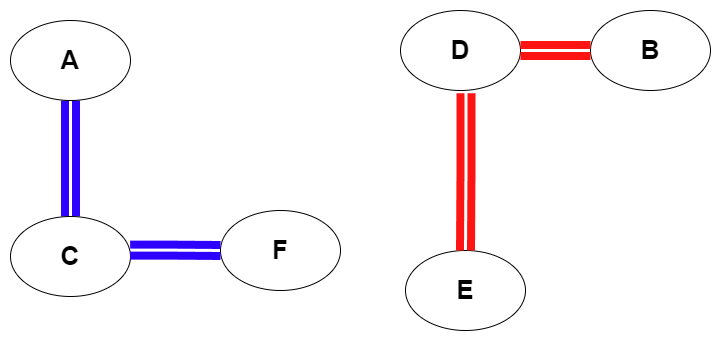
\includegraphics[width=15cm]{obrazky-figures/nn.png}
\caption{Nejbližší sousedi}
\label{fig:nn}
\end{figure}
\subsection{Volba parametrů}\label{sec:params}
Volba parametrů je velmi důležitou částí ACO algoritmu. Správnou volbou parametrů můžete urychlit nalezení kvalitního řešení. Je to poměrně kritická část ACO, jelikož parametry mají velký vliv na řešení. Špatnou volbou parametrů můžete dokonce z funkčního algoritmu udělat velmi špatný algoritmus. Můj program již má předem nastavené parametry, které jsem vyladil dlouhým testováním programu. Přednastavené parametry jsou uvedeny na obrázku \ref{fig:settings_ACO} v levé části. Zde se zaměříme na každý z nich a popíšeme, co dělá, jaká by měla být optimální hodnota a jaké jsou možné hodnoty.
Jednotlivé informace o parametrech jsou čerpány z \cite{Li2016}.
\begin{itemize}
    \item \textbf{$\alpha$} -- Reprezentuje důležitost vyloučeného feromonu na cestě. Pokud by byl parametr nastaven jako příliš velké číslo, mravenci by měli tendenci volit ty samé cesty jako předchozí, což by vedlo k silnější spolupráci mezi mravenci. Na druhou stranu, to nemusí být nutně výhoda, protože algoritmus by mohl zůstat pouze v lokálním řešení a nenajít žádné lepší. Pokud by ale hodnota byla příliš malá, rychlost konvergence ACO by se zpomalila, bez ohledu na to, že lze globální vyhledávací schopnost algoritmu zlepšit. Optimálně nastavená hodnota je podle mě (0.7,2.0).
    \item \textbf{$\beta$} -- Reprezentuje faktor viditelnosti na cestě. Pokud je hodnota příliš velká, algoritmus se bude blížit řešení pomocí Nearest Neighbour, protože se budou vybírat nejlepší cesty na základě viditelnosti, která je přímo úměrná vzdálenosti mezi místy. To může vést k uvíznutí v lokálním řešení. Na druhou stranu, pokud je hodnota příliš nízká, cesty s velkou vzdáleností budou stejně atraktivní jako ty s malou, což může vést k stagnaci algoritmu. Podle mého názoru je optimální rozsah hodnot (1.0,35.0).
    \item \textbf{$\rho$} --  Koeficient odpařování feromonu vyjadřuje míru odpařování feromonu a odráží míru vzájemného ovlivňování mezi mravenci. Obecně by měla být hodnota dostatečně vysoká, aby účinně bránila nekonečnému hromadění feromonu. Pokud je hodnota příliš malá, může se snížit globální vyhledávací schopnost ACO. Naopak, pokud je příliš vysoká, může se zlepšit globální vyhledávací schopnost ACO, ale rychlost konvergence bude pomalá. Optimální rozsah se pohybuje někde mezi (0.1,0.3). Hodnota by neměla být větší než 1 a menší než 0.
    \item \textbf{Q} -- Intenzita feromonu představuje celkové množství feromonu na jednotlivých hranách grafu a ovlivňuje rychlost konvergence ACO. Pokud je hodnota příliš vysoká, koncentrace feromonu bude příliš vysoká a algoritmus může upadnout do lokálního optima. Naopak, pokud je hodnota příliš nízká, rychlost optimalizace bude pomalá. Podle mého názoru je optimální rozsah mezi (2000, 50000).
    \item \textbf{q0} -- Vyjadřuje konstantu, s jakou pravděpodobností se zvolí ta nejpravděpodobnější cesta. Tento prvek je důležitý, protože pokud by byl nastaven na velkou hodnotu, naše řešení by se blížilo k řešení pomocí Nearest Neighbour. Nicméně, tento parametr v ACO nehraje klíčovou roli a může být klidně nastaven na hodnotu 0, pokud ho nechcete použít. Jedná se pouze o vylepšení, které pomáhá najít lepší řešení rychleji. Optimální rozsah pro tuto konstantu je někde mezi 0 a 0.5. Minimální hodnota je 0 a maximální hodnota je 1. Funguje to následovně: Nejprve zvolíme konstantu q0, například 0.4. Poté náhodně vygenerujeme číslo q v rozsahu (0,1). Pokud je $q$ menší než $q0$, zvolíme nejpravděpodobnější cestu. Pokud je $q$ větší než $q0$, volíme cesty podle pravděpodobností.
\end{itemize}





\section{MyAlgo} 
Rozhodl jsem se navrhnout vlastní algoritmus, jelikož ACO byla prakticky nepoužitelná pro více než 1000 míst a kvalita řešení nebyla zrovna uspokojivá, i s využitím 2-opt algoritmu pro optimalizaci řešení. Původně jsem chtěl zvolit Artifical Atom Algorithm jako druhý hlavní algoritmus, ale po shlédnutí výsledků, i když byl algoritmus schopný nalézt většinou optimální řešení do 50 míst, trvalo to asi 100 sekund. Což bylo ještě pomalejší než ACO. Původní myšlenky, které mě napadly, byly, že bych mohl implementovat přehazování míst na základě pravděpodobnosti, která by fungovala podobně jako v ACO (závisela by na délce celkové cesty a délce cesty od místa A do místa B), ale pouze by se mohla vylepšovat a přehodil by se do lepšího řešení. Zde jsem si uvědomil, že by se algoritmus mohl hodně rychle zaseknout a nenalézt lepší cestu, takže jsem ani nezačal s implementací.

\subsection{Myšlenka}
Základní myšlenku jsem převzal asi z nejlepšího algoritmu na řešení problému obchodního cestujícího, konkrétně z algoritmu \textbf{lin–kernighan heuristic}. Tento algoritmus se snaží vylepšit řešení pomocí prohození míst. Mě napadlo, že by bylo dobré vygenerovat optimální řešení pro nejbližších x míst a poté je spojit dohromady s použitím hranic. Avšak, protože bychom mohli uváznout v lokálním optimu, rozhodl jsem se nebrat v úvahu všechna místa, ale vždy vybrat určité místo jako začátek a přidávat další místa k němu postupně, abychom procházeli různé možnosti se stejnými místy. Z toho mi vyplynulo, co bych potřeboval implementovat. Vždy zvolím místo, které jsem nezvolil jako začátek, a přidám k němu několik nejbližších sousedů. Poté vypočítám "optimální řešení" mezi nimi. Pokud je nové řešení lepší než původní, přepojím body. I když je myšlenka jednoduchá, implementace byla poměrně obtížná, zejména v počítání vzdáleností v přepojovaných místech a volbě nových hranic. Také jsem si uvědomil, že pokud například počítám vylepšení pro 5 míst, mohu přepojit 5 míst, ale optimální cesta pro 4 místa by mohla být vylepšena, ale pro 5 míst ne. Proto přidávám místa postupně a vybírám to nejlepší možné vylepšení z nich.

\subsection{Popis algoritmu}
\begin{enumerate}
\item Nastaví se čítač \textbf{s} na 0 a uloží se počáteční řešení.
\item Nastaví se aktuální řešení problému na počáteční řešení.
\item Dokud se zlepšení dá dosáhnout, volá se jádro algoritmu s počáteční hodnotou sousedů + \textbf{s}.
\item Pokud se zlepšení nedá dosáhnout, volá se jádro algoritmu s prostřední hodnotou sousedů.
\item Aplikuje se na problém 2-opt algoritmus pro optimalizaci.
\item Uloží se trasa a aktuální délka trasy.
\item Pokud je čítač \textbf{s} větší nebo roven počtu počátečních řešení, pokračuje se na bod \textbf{7}. Pokud ne, inkrementuje se čítač \textbf{s} a vrátí se na bod 2.
\item Vybere se nejlepší počáteční trasa.
\item Pro nejlepší vybranou počáteční trasu se volá jádro algoritmu s posledním počtem sousedů, dokud se zlepšuje.
\end{enumerate}

\subsection{Popis jádra algoritmu}
\begin{enumerate}
\item Začne se iterovat nad všemi místy tak, aby se každé prošlo právě 1x.
\item Pro aktuální místo se zjistí levá a pravá hranice.
\item Vypočítá se vzdálenost místa po odpojení od jeho hranic.
\item Uloží se aktuální místo z bodu \textbf{1} jako počáteční.
\item Vytvoří se struktura, která ukládá novou část cesty, a vloží se tam počáteční místo.
\item Nastaví se čítač \textbf{z} na 0.
\item Zvolí se nejbližší soused, buď nejbližšího k počátečnímu místu, nebo místu aktuálnímu. Souseda nastavíme jako aktuální místo.
\item Kontrola, jestli místo není hranicí. Pokud je, musí se vypočítat vzdálenost po přepojení hranic.
\item Pokud místo není hranice, musí se vypočítat vzdálenost po odpojení od jeho hranic.
\item Odstraní se aktuální místo.
\item Do struktury pro novou část cesty se vloží aktuální hranice a aktuální místo.
\item Na novou část cesty se aplikuje 2-opt algoritmus.
\item Z struktury pro novou část cesty se oddělí hranice, ale zároveň se nechají ve výsledku pro část nové cesty.
\item Spočítá se vzdálenost nové cesty a uloží se vzdálenost a nová část cesty.
\item Pokud je čítač \textbf{z} větší nebo roven počtu nastavených sousedů, pokračuje se na další bod. Pokud ne, inkrementuje se čítač \textbf{z} a vrátí se na bod \textbf{7}.
\item Vybere se nejlepší cesta dle vzdálenosti.
\item Z té se vytvoří nová cesta, která se vytváří z cesty, ve které je odpojeno určité množství míst, a ten samý počet stejných míst tvoří novou část cesty.
\end{enumerate}


\subsection{Přepojování míst}\label{sec:places changes}
Jednou z klíčových částí algoritmu je přepojování míst a výpočet vzdáleností po přepojení. Počítání celkové vzdálenosti a provádění změn v poli je totiž v porovnání s tímto způsobem extrémně výpočetně náročné. Abychom mohli přepojování míst použít pro všechna místa s použitím hranic, musíme vytvořit cyklus z pole míst, kde místo na indexu 0 bude mít jako levého souseda místo na posledním indexu a místo na posledním indexu bude mít jako pravého souseda místo na nultém indexu. Prvním krokem je zvolit nějaké místo, které ještě nebylo zvoleno, řekněme místo A. Předpokládejme, že máme množinu míst [A, B, C, D, E]. Pro místo \textbf{A} musíme zvolit levého souseda (místo \textbf{E}) a pravého souseda (místo \textbf{B}). Poté musíme spočítat vzdálenost odpojení místa \textbf{A} od \textbf{E} a \textbf{B}. To zahrnuje cestu z místa \textbf{E} do \textbf{A} a cestu z místa \textbf{A} do \textbf{B}. Tuto vzdálenost nazýváme například \textbf{vzdálenost hranic}. Poté vybereme nejbližší místo k místu \textbf{A}, což v tomto případě bude místo \textbf{E}.
Jelikož místo \textbf{E} je zároveň levá hranice posunu levou hranici na místo \textbf{D}. Tím že je místo \textbf{E} je levá hranice znamená, že nemá pravého souseda toho už jsme odpojili u vzdálenosti hranic. Proto jediné co musíme spočítat je vzdálenost po odpojení místa \textbf{E} od jeho levého souseda místa \textbf{D}, což bude vzdálenost z místa \textbf{E} do \textbf{D}. Pokračuji dále, tím že vyberu další místo nejblíže místu \textbf{A}, které jsem ještě nevybral, což bude místo \textbf{C}. Jelikož místo \textbf{C} není pravá ani levá hranice, musím jeho vzdálenost po odpojení spočítat tak, že vezmu rozdíl vzdáleností přepojení pravé hranice místa C do levé hranice místa C a odpojení místa \textbf{C} od hranic místa C. To je rovno cesta z \textbf{B} do \textbf{D} - cesta z \textbf{B} do \textbf{C} - cesta z \textbf{C} do \textbf{D}.
Poté s použitím hranic vytvořím nejlepší řešení přeskládáváním míst [A,C,E]. Řešení, které dostanu bude vypadat například jako [E,A,C]. Vypočítáme vzdálenost po připojení, což bude vzdálenost levé hranice \textbf{D} do místa E + vzdálenost řešení + vzdálenost místa C do pravé hranice \textbf{B}. Vzdálenost řešení je vzdálenost z místa \textbf{E} do \textbf{A} + vzdálenost z \textbf{A} do \textbf{C}. Na takto malém příkladu se to může zdát počítat jako zbytečné, ale když máte pro tisíce míst spočítat celkovou vzdálenost je to časově náročnější než pouze vzdálenost po přepojení. Ještě by se museli dělat změny v poli kterým se vyhneme, pokud přepojování míst nevylepší řešení. Na obrázku \ref{fig:Places changed} můžeme vidět přesně to co jsem zde napsal, jak se z levého grafu stane ten pravý. 

\begin{figure}[H]
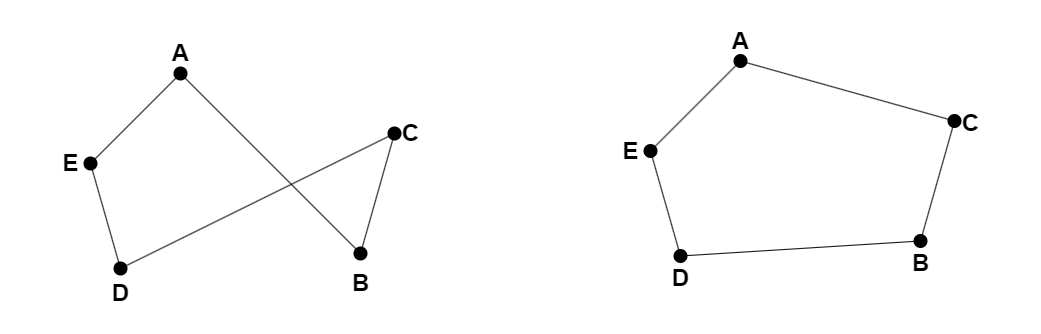
\includegraphics[width=15cm]{obrazky-figures/change_points.png}
\caption{Přepojení míst}
\label{fig:Places changed}
\end{figure}

\subsection{Problémy s uváznutím v lokálním optimu}\label{sec:loc min}
Jelikož je jádro algoritmu poměrně rychlé, pro 4000 míst za 10 vteřin zvládne vyřešit problém s 10 nejbližšími sousedy. Pro 1 souseda a 4000 míst je to pod vteřinu. Pokud použijeme více sousedů, řešení se většinou zlepší. Jenže jsem si všiml jedné věci, algoritmus je hodně závislý na prvotním generovaném řešení. Když je špatné, uvízne a už se nezlepší. Proto jsem se rozhodl aplikovat způsob postupného vylepšování cesty postupným zvyšováním počtu sousedů, což opravdu má velký vliv na kvalitu řešení. Místo toho, abych hned aplikoval například 60 sousedů, aplikuji nejdříve 1 souseda, pak 2, a poté 3. Můžeme tomu říkat \textbf{první nejbližší sousedi}, protože většinou platí, že čím víc sousedů, tím lepší řešení. Musím pro každé řešení prvního nejbližšího souseda nějak dorovnat řešení "aby to bylo fér". Proto každé řešení prvního nejbližšího souseda vezmu a vylepším stejným počtem sousedů, například 10, poté na každé řešení aplikují 2-opt algoritmus a vyberu to nejlepší. Nakonec se snažíme co nejvíce vylepšit řešení, takže zvýšíme hodnotu sousedů, například na 60.
\subsection{Rozdělení problému na segmenty}\label{sec:segments}
Všiml jsem si, že pokud náhodně generuji počáteční cestu a následně aplikují MyAlgo, je možné dostat lepší řešení. Abych využil tuto vlastnost a zároveň neřešil celý problém najednou, rozhodl jsem se rozdělit ho na menší podproblémy a ty postupně zlepšovat. Když místa v podproblému náhodně zamíchám a aplikují MyAlgo, pokud je aktuální část řešení horší než nově vygenerovaná, nahradím ji. I když tato úprava zní jednoduše, celé jádro algoritmu a všechny pomocné funkce se musely předělat. Jádro algoritmu je na bázi cyklu, jak je zmíněno v \ref{sec:places changes}, kde v podstatě neexistuje nejpravější a nejlevější prvek. Ale pokud vezmeme jen určitou část problému, musíme vzít i nějaké hranice segmentu. Po překonání velikosti segmentu (myslím tím, když chceme dostat pravý prvek od nejpravějšího prvku v segmentu nebo levý od nejlevějšího), jsou tyto hranice nutné. Pokud tam tyto hranice nebyly, v podstatě by to znamenalo, že řešení, které nám jádro vrátí, nemusí vůbec zapadat do celkového problému, protože bychom tam nepočítali vzdálenost při napojení do celkového řešení. Všechny funkce se musely předělat, například funkce pro vytváření nové cesty, pokud je zlepšení vkládala novou cestu vždy po levé hranici. Jenže pokud použijeme jen určitý segment a naše levá hranice je zároveň hranice segmentu, kterou nemohu měnit, nemůžu vložit řešení v rámci podproblému, kde není hranice segmentu. Pokud je levá hranice zároveň hranice levého segmentu, tak na začátek, pokud pravého, tak na konec. Pro představu je to vyobrazeno na obrázku \ref{fig:Segments}. Kde písmena značí označení, v reálném programu se nepracuje s tak malým počtem míst a segment náhodně zamícháváme pouze pro představu. Písmeno A značí původní spojení míst. Představme si, že pro toto spojení je segment, který chceme upravovat, vyobrazen růžově a jeho hranice modře. Písmeno B označuje skupinu bodů, kterou dostaneme v rámci jádra algoritmu. Levá a pravá hranice jsou vybarveny černou barvou a jsou to místa 1 a 5. Zároveň si můžeme všimnout, že levá hranice je zároveň hranicí segmentu. Poté aktivujeme 2-opt. Jak vidíte, nepřehazuje se hraniční body a dostaneme řešení C. Nakonec vyměníme segment v celkovém řešení, pokud dojde ke zlepšení, a to je reprezentováno řešením D. 

\begin{figure}[H]
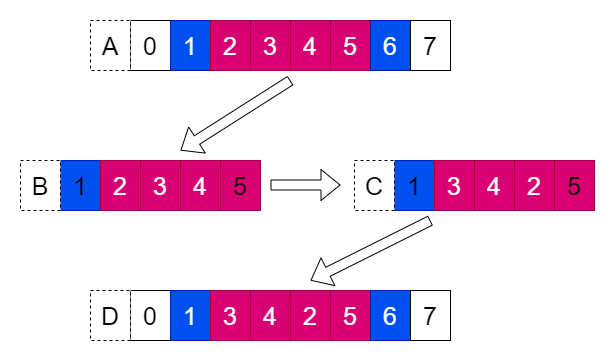
\includegraphics[width=15cm]{obrazky-figures/segments.png}
\caption{Segmenty}
\label{fig:Segments}
\end{figure}

\subsection{Náměty na zlepšení algoritmu}
První možností, která by určitě fungovala, je \textbf{využití vláken}. Nabízí se zde několik způsobů, jak vlákna využít. Jak je zmíněno v sekci \ref{sec:loc min}, generuji nějaký počet prvotních řešení, ze kterých vybírám to nejlepší a až poté aplikuji větší rozsah sousedů. Skupina prvotních řešení není na sobě nijak závislá, jen se vybírá to nejlepší. Zde se přímo nabízí využití paralelizace pro každé z prvotních řešení.

Další možností by mohlo být využití při segmentech, jelikož jednotlivé segmenty nejsou na sobě závislé. Tato myšlenka napadne asi každého. Další způsob využití vláken by mohl být například v jádru algoritmu, kde používám pro volbu kandidátů pouze nejbližšího souseda k aktuálnímu místu a k počátečnímu. Například jedno vlákno by mohlo využívat tuto techniku a druhé nějakou pokročilejší techniku, například volbu mezi nejbližšími sousedy na základě pravděpodobností. Poté by se použil vždy ten lepší výsledek. S tím souvisí i další nápad, který mě napadl, a to je v podstatě vracení řešení na nějaký určitý záchytný bod, pokud dojde k uváznutí a není způsob, jak se zlepšit. Následně by se řešení generovalo jiným způsobem, například metodou vkládání místa nebo skupiny míst na lepší pozici, což je v podstatě opačný způsob fungování algoritmu. Dokonce jsem ji již pro 1 místo implementoval. Způsobů, jak zlepšit aktuální řešení, je určitě hodně. Kvalita řešení by se určitě zlepšila i využitím více opt algoritmu, například pro jednotlivé segmenty, ale implementace například 5-opt algoritmu není jednoduchá, aby byla zároveň efektivní a netrvala příliš dlouho. Jedinou verzi, kterou jsem našel, již implementovanou byla součástí LKH algoritmu a je popsaná zde: \cite{helsgaunkopt}.







\chapter{Návrh a implementace algoritmů}
\section{Ant Colony Optimization Algorithm}
Původně jsem se rozhodl algoritmus implementovat v jazyce Python, ale kvůli absenci paralérního zpracování vláken v jazyce jsem algoritmus přepsal do jazyka C++ a ještě ho nějak vylepšil. Implementaci v jazyce Python zde popisovat nebudu, jelikož ji v programu nevyužívám.  
\subsection{Zpracování vstupního souboru}\label{sec:start file}
Vstupem algoritmu je soubor algo\_inputN.txt kde N je číslo jádra na kterém algoritmus běží.
Prvních 11 řádků souboru je nastavení algoritmu neboli parametry, které jsme zvolili. Řádky které následují reprezentují místa. Místo si můžeme představit jako nějakou strukturu, která má nějaké unikátní označení \textbf{ID}. Dále místo obsahuje souřadnice \textbf{X} a \textbf{Y}. 
A list vzdálenosti do ostatních míst. Přesně v tomto pořadí se nachází i na řádcích v souboru algo\_inputN.txt. Takže funkce \textbf{parse\_file\_to\_places()} přečte soubor a zpracuje ho do proměnných reprezentující parametry ACO. A vytvoří dynamické pole s místy, které naplní konkretním počtem míst co je v souboru.  
\subsection{Přednastavení feromonů}
Struktura místa bude kromě dynamického pole pro vzdálenosti do ostatních míst obsahovat i dynamické pole pro jejich $\tau$ množství vyloučených feromonů na cestě do ostatních míst. Počáteční nastavení hodnoty na zvolené množství $\tau0$ se uskuteční v funkci \textbf{parse\_file\_to\_places()}. Dále, aby neměly všechny cesty stejné množství $\tau$ a zrychlila se tím i rychlost algoritmu, použije se funkce \textbf{setup\_nn\_tau()}. Funkce nastaví počáteční feromony pomocí Nearest Neighbour algoritmu. Konkrétně se zvolí počáteční místo, které ještě nebylo vybráno. A pomocí nastavených iterací a délky míst v Nearest Neighbour se pomocí tohoto algoritmu přenastaví $\tau$. Oproti normálnímu přenastavování $\tau$ zde není žádné vyprchávání feromonů, pouze se pomocí funkce \textbf{setup\_tau\_start\_NN()} přičte $\Delta\tau$ k $\tau$, kde $\Delta\tau = \frac{Q}{trasa}$. Q je předem nastavený parametr a trasa je celková trasa Nearest Neighbour algoritmu.
\subsection{Vytvoření agentů}
Pomocí funkce \textbf{setup\_threads()} jsou vytvořena jednotlivá vlákna pro agenty s počtem vláken, který byl nastaven. Poté se v funkci \textbf{created\_agent()}, která běží jako samostatné vlákno, začne iterovat v počtu nastavených iterací. V každé iteraci jsou volány 3 další funkce.
\begin{itemize}
\item \textbf{agent\_chose\_path} -- Lze říct, že funkce je srdcem ACO, neboť se v ní odehrává samotné procházení míst algoritmem. Nejprve se náhodně zvolí začínající místo. Poté se začne iterovat od 0 do celkového počtu míst - 1. První krok spočívá výpočtu součtu všech viditelností a hodnoty $\tau$ z aktuálního místa do ostatních míst za pomoci funkce \textbf{setup\_visibility\_tau}. Konkrétně se jedná o tuto část vzorce:
\begin{center}
\scalebox{1.5}{$ SUM = \sum_{0}^{N}\left[\tau_{i l}\right]^\alpha\left[\eta_{i l}\right]^\beta$}
\end{center}
Poté se aktuální místo odstraní z pole nenavštívených míst a začne se iterovat od 0 do velikosti pole nenavštívených míst -1. V každé iteraci se spočítá viditelnost a hodnota $\tau$ pro konkrétní trasu a vypočítá se pravděpodobnost cesty z aktuálního místa i do dalšího nenavštíveného místa. Toto vyplývá z následujícího vzorce:
    \begin{center}
        \scalebox{1.5}{$p_{i j}=\frac{\left[\tau_{i j}\right]^\alpha\left[\eta_{i j}\right]^\beta}{SUM}$}
    \end{center}
    Poté, kdy skončí iterování v nenavštívených místech a máme uložené všechny potřebné pravděpodobnosti tras, náhodně vybereme číslo q z rozmezí (0,1). Pokud je q menší než q0, nastavíme aktuální místo na to s nejvyšší pravděpodobností. V opačném případě vybereme aktuální místo z nenavštívených míst na základě pravděpodobnosti. Poté se přičte vzdálenost z posledního navštíveného místa do aktuálního místa. Tímto končí cyklus, který probíhal až do počtu míst - 1. Nakonec se ještě přičte vzdálenost zpět do prvního místa a první místo se vloží do seznamu navštívených míst. Funkce vrátí strukturu, kde je uložena trasa navštívených míst a celková vzdálenost.
    \item \textbf{agent\_update\_tau} --
     Funkce slouží k aktualizaci sdílených feromonů mezi vlákny. Nejprve se použije zámek, protože $\tau$ je sdílená proměnná pro všechny vlákna a přístup k proměnné více vlákny najednou by mohl způsobit problémy. Navíc by hodnoty feromonů nebyly aktualizovány s aktuálními hodnotami. Poté se vypočítá $\delta\tau=\frac{Q}{D}$. Kde \textbf{D} je vzdálenost cesty v aktuálním vláknu a v rámci iterace. \textbf{Q} je konstanta, kterou jsme nastavili. Poté se přičte $\delta\tau$ ke všem cestám, které jsme v aktuálním vláknu v rámci iterace navštívili, a zámek se odemkne.
    
    \item \textbf{agent\_check\_best\_distance} --
    Funkce slouží pouze k udržení nejlepší cesty a vzdálenosti. Zase zde musíme použít zámek, protože nejlepší cesta a vzdálenost jsou globální proměnné. Funkce pouze kontroluje, zda je aktuální cesta lepší než nejlepší cesta; pokud ano, uloží se jako nová nejlepší cesta.
    
    \item \textbf{pheromone\_evaporation} --
    Funkci volá pouze jeden agent, a to ten poslední. Slouží k vypařování feromonů. Je jedno, zda jdu z místa [A] do [B] nebo z [B] do [A], protože ve funkci neprocházíme všechny cesty. Navíc je cesta z [A] do [A] irelevantní. Iterujeme pouze od determinantu matice a kopírujeme hodnoty na druhou stranu matice, kde jsou hodnoty stejné ([A][B] == [B][A]). Vypařování se počítá jako $\tau=\tau(1-\rho)$, kde $\rho$ je zvolená konstanta.
\end{itemize}
    \subsection{Aktivace 2-opt} 
     Pro optimalizaci cesty a zlepšení řešení používám 2-opt algoritmus, který většinou odstraní křížení cest v řešení. Tento algoritmus se volá s nejlepší nalezenou cestou v ACO a pokouší se ji vylepšit.
    \subsection{Zapsaní nejlepších výsledku do souboru}\label{sec:best file}
    Poslední věcí, která se odehraje, je zapsání nejlepší vzdálenosti do souboru \\ \textbf{best\_pathN.txt}, kde \textbf{N} je číslo jádra, na kterém algoritmus běží. Soubor se otevře a zapíše se na jeden řádek navštívená místa oddělená mezerami a na druhém řádku bude vzdálenost cesty. 

\section{MyAlgo} 
MyAlgo je taky pro zlepšení rychlosti implementovaný v jazyce C++. Skládá se v podstatě z dvou hlavních funkcí \textbf{start\_algo}, která koordinuje algoritmus. A funkce \textbf{core}, která je v podstatě jádro algoritmu. Tyto funkce využívají různých vedlejších funkcí. Ještě se zde nachází funkce, která používá místo celého řešení pouze segmenty \textbf{core\_for\_segment}. Dále se v algoritmu nachází i funkce \textbf{start\_core\_insertion}, kterou nevyužívám, protože nezlepší řešení. Rychlost a princip algoritmu spočívá v myšlence, pokud je přepojení lepší, tak teprve potom udělej změny v poli. Funguje zde stejně načítání míst \ref{sec:start file} a zápis nejlepšího řešení \ref{sec:best file} jako v ACO. S jediným rozdílem a to, že zde nepoužíváme jádra procesu. Popíši zde hlavní funkce algoritmu například nebudu zde popisovat funkce pro segmenty, jelikož fungují na stejném principu jako ty normální a rozdíl je už vysvětlený v teorii a taky funkce, které nepoužívám je jich tam hodně zkoušel jsem, jak bych v algoritmu fungovali, ale neosvědčili se mi. Na druhou stranu jdou zlepšit, tak jsem je nechtěl mazat například best5 může být použita pro víc prvků ne jen pro 5. 
\subsection{start\_algo}
Funkce funguje jako koodrinátor algoritmu. Má 3 hlavní úkoly:  
\begin{itemize}
    \item \textbf{Vygenerovat určitý počet počátečních řešení} - Nejprve se zavolá jádro algoritmu s počátečním počtem sousedů. Pokud se řešení zlepšuje, stále se volá jádro algoritmu s tímto počtem sousedů. Poté se opakuje tento postup s prostředním počtem sousedů a opět se hledá zlepšení. Nakonec se pokusí zlepšit celé řešení pomocí 2-opt algoritmu. Tento postup se opakuje s postupně větším počtem počátečních sousedů, až se dosáhne nastaveného počtu.
    \item \textbf{Vybrat nejlepší z počátečních řešení a zlepšit ho} - nejlepší z počátečních řešení se vybere a pokusí se zlepšit voláním jádra algoritmu s posledním počtem sousedů. Zase se používá strategie, dokud se řešení zlepšuje voláme jádro s tímto počtem sousedů. 
    \item \textbf{Použití segmentů} Zde se volá jádro pro segmenty, je potřeba si i představit, jak část řešení bude fungovat například pokud se volá segment velikosti 120 je zbytečné volat segment velikosti 60. Po testovaní jsem přišel na docela pěkné velikosti segmentů, které skoro vždy zlepší výsledek od 120 do 102 vždy o 3 místa, aby se co nejvíc kryly. 
\end{itemize}
\subsection{core}
Funkce je srdcem algoritmu, iteruje přes všechny místa co máme. V podstatě se snaží v každé iteraci vybírat za pomocí nejbližších míst kandidáty, které vloží vedle sebe a s nimi za pomoci 2-opt algoritmu zlepší řešení. Funkce v každé iteraci pro aktuální místo dělá následující kroky:
\begin{itemize}
    \item Za pomocí funkce cycle zvolí index levé a pravé hranice.
    \item Indexy použije v aktuální cestě a zjistí levé a pravé hranice.
    \item Spočítá vzdálenost po odpojení místa nad kterým iterujeme v původním spojení.
    \item Začíná iterovat nad zvoleným počtem nejbližších sousedů.
    \item Vybere z postupného iterovaní nad nejbližšími sousedy nejlepší výsledek.
    \item Pokud je nejlepší výsledek horší jak aktuální cesta použije se aktuální cesta, jinak se vytvoří nová cesta s nejlepším výsledkem za pomocí funkce construct\_new\_path.
\end{itemize}
Jak je zmíněno v čtvrtém bodě, je zde důležitá věc, a to, že se začíná iterovat nad zvoleným počtem sousedů. Zde jsou důležité kroky, které se musí v iteraci odehrát:

\begin{itemize}
\item Vybere se místo, buď nejbližší nevybraný soused od předchozího vybraného místa, nebo od místa, nad kterým iterujeme.
\item Vždy musíme zkontrolovat, jestli místo vybrané pomocí nejbližšího souseda není levá nebo pravá hranice, a to za pomocí funkce check\_border. Zde je třeba si představit, jak to bude fungovat a proč tady vlastně odlišujeme hranice, jak je zmíněno v předchozím seznamu v bodě 3. Spočítáme vzdálenost aktuálního místa po odpojení, což znamená, že pravá a levá hranice nejsou z jedné strany napojené. Takže pro hranice jen odečteme jednu stranu a musíme hranice nahradit novou hranicí. Pokud místo není hranice, musíme od jejího levého a pravého místa odpojit a tyto místa spojit k sobě, a k tomu využíváme funkci calculate\_distance\_after\_remove\_point.
\item Musíme zkonstruovat cestu mezi místy, které jsme už odpojili, a to včetně levé a pravé hranice. Zde si musíme představit, že řešení vkládáme mezi ně.
\item Nakonec spočítáme vzdálenosti mezi místy, které nám vrátí 2-opt algoritmus, a zjistíme, jestli není v iteraci sousedů nejlepší. Pokud je, uložíme si ji.
\end{itemize}
    \subsection{cycle}
Jednoduchá pomocná funkce, která z pole vytvoří cyklus. Volá se tak, že ji předáme aktuální index, informaci o tom, jestli chceme pravý nebo levý index od aktuálního indexu a velikost cesty. Pokud chceme získat pravý index a zároveň je aktuální index poslední v poli, vrátíme první index. Stejně tak, pokud chceme levý index od prvního indexu, vrátíme ten poslední v poli. V ostatních případech získáme pravý index tak, že přičteme k aktuálnímu indexu 1 a levý index tak, že od aktuálního indexu odečteme 1.

\subsection{calculate\_distance\_after\_remove\_point}
Funkce, která má spočítat vzdálenost po odebrání místa od jeho levé a pravé hranice a spojení hranic k sobě. K určení pravé a levé hranice použijeme funkci cycle. Poté jen spočítáme vzdálenost jako součet vzdálenosti od levé hranice ke zvolenému místu, vzdálenosti od zvoleného místa k pravé hranici a odečteme vzdálenost od levé hranice k pravé hranici.

\subsection{construct\_new\_path}
Funkce, která vytvoří novou cestu z části cesty hranic a staré cesty. Nejprve si vytvoříme cestu takovou, která neobsahuje novou část cesty ze staré cesty, kromě levé hranice, která je uložena na nultém indexu. Poté za levou hranici vložíme novou část cesty a vrátíme novou cestu.


    


\chapter{Struktura a implementace programu}
\section{Výběr jazyků}
Pro svou jednoduchost a rychlost implementace jsem se rozhodl použít jazyk Python, který jsem použil na části programu, kde rychlost nebyla hlavním faktorem, například pro grafické rozhraní a skriptu, který slouží k využití všech jader procesoru. Pro druhou část programu, kde byla rychlost velmi důležitým faktorem, jsem se rozhodl použít jazyk C++. Také jsem zvažoval, zda použít knihovnu Numba pro implementaci algoritmů. Numba je just-in-time kompilátor pro jazyk Python, který nejlépe funguje s kódem, který využívá pole a funkce v NumPy, a s cykly. Nejběžnějším způsobem použití Numba je pomocí dekorátorů, které lze aplikovat na funkce, aby se Numba naučila, jak je optimalizovat. Pokud je poté zavolána funkce s dekorátorem, je přeložena do strojového kódu pro okamžité vykonání a celý nebo část kódu může následně běžet rychlostí nativního strojového kódu \cite{numbaDocs}. Rozhodování, jestli zvolím jazyk Python společně s knihovnou Numba nebo jazyk C++, bylo složité, ale nakonec jsem zvolil jazyk C++, i díky srovnání rychlosti při paralelizaci, které je vidět na pravé straně grafu v obrázku \ref{fig:Cpp vs Numba}, převzatém z \cite{Comparing}. Tento graf ukazuje rychlost jednotlivých jazyků při řešení problému N dám.

Implementoval jsem také Ant Colony Optimization Algorithm a Nearest Neighbor Algorithm v jazyce Python. Jedním z problémů při použití Pythonu je problém s využíváním vláken. Globální zámek interpretu Pythonu, zvaný GIL, je mutex (nebo zámek), který umožňuje pouze jednomu vláknu ovládat interpret Pythonu. To znamená, že pouze jedno vlákno může být v režimu spuštění v jakémkoli bodě v čase. Dopad GIL není viditelný pro vývojáře, kteří spouštějí jednovláknové programy, ale může být úzkým místem výkonu v programování vázaném na procesor a vícevláknovém kódu. Informace převzatá z \cite{RealPythonGIL}.
Celkově to zabraňuje paralelizaci jednotlivých úloh na úrovni vláken. Jelikož v \textbf{Ant Colony Optimization Algorithm} každého mravence reprezentuje vlákno, tak nedává smysl Python využívat. 
\begin{figure}[H]
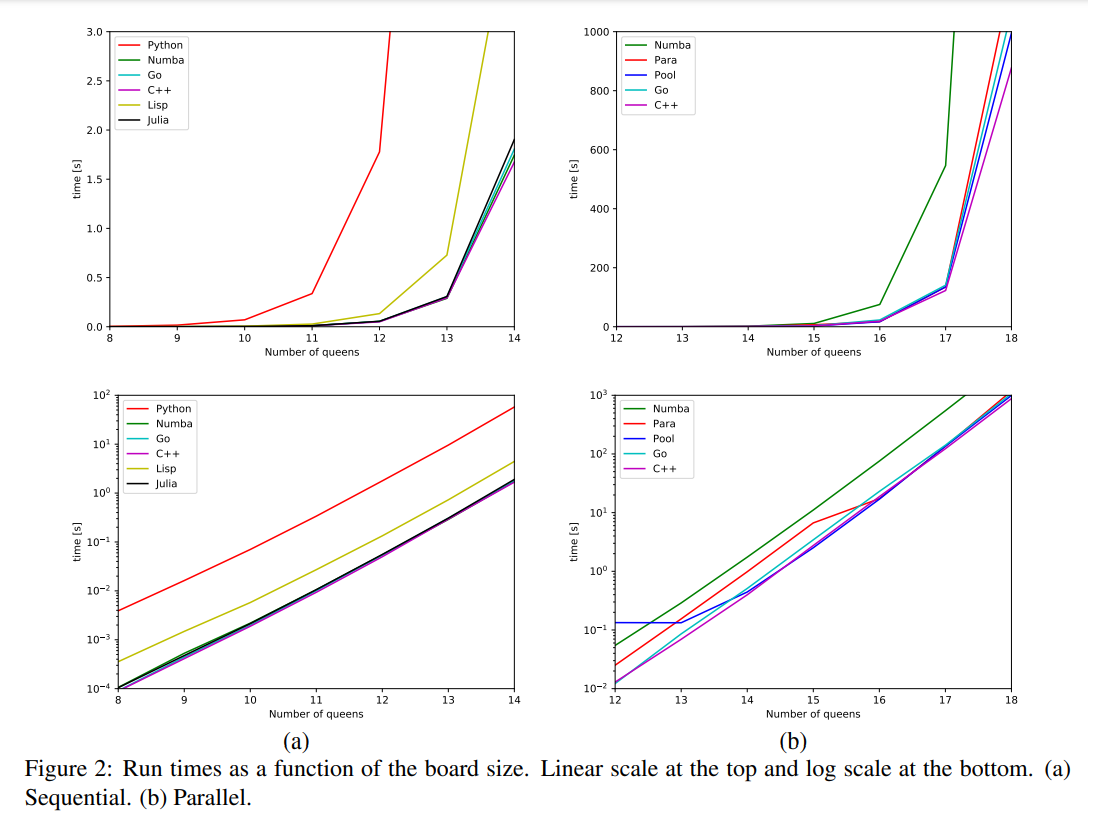
\includegraphics[width=15cm]{obrazky-figures/cpp_vs_numba.png}
\caption{C++ vs Numba}
\label{fig:Cpp vs Numba}
\end{figure}


\section{Struktura aplikace}
Jednotlivé části aplikace jsou zobrazeny na obrázku \ref{fig:struktura ap}. Po spuštění aplikace se zobrazí \textbf{grafické uživatelské rozhraní}, které umožňuje zobrazovat místa a jejich cesty a dokáže místa i generovat. Po stisknutí tlačítka \textbf{Solve} se grafické uživatelské rozhraní rozdělí na 2 vlákna. V jednom bude běžet grafické uživatelské rozhraní a v druhém se za pomocí python interpretu spustí \textbf{Prostředník}. Prostředník nejprve přeloží algoritmus za pomocí optimalizačního přepínače \textbf{O3}. O3 instruuje kompilátor, aby optimalizoval výkon generovaného kódu a ignoroval velikost generovaného kódu, což může vést k většímu objemu kódu \cite{ARMOptimization}. Následně prostředník zjistí počet jader systému a poté ze souboru algo\_input přečte, kolik jader uživatel chce použít. Pokud je počet jader, které chce uživatel použít, větší než reálný počet jader procesoru, prostředník sníží zvolený počet na maximální možný. Poté se na každém jádru spustí algoritmus. Na obrázku \ref{fig:struktura ap} je vidět, jak by to fungovalo, pokud by byl počet zvolených jader 3 (samozřejmě by ty jádra musela být k dispozici).
\begin{figure}[H]
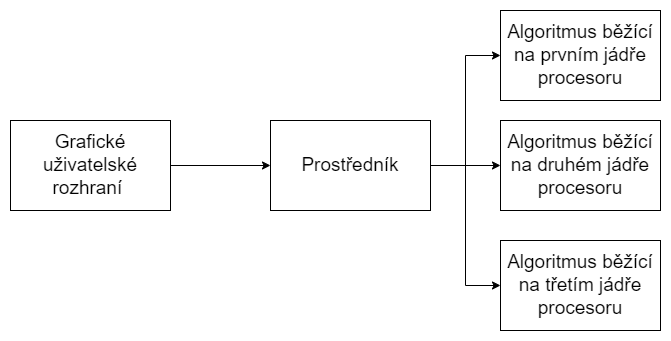
\includegraphics[width=15cm]{obrazky-figures/struktura_ap.png}
\caption{Struktura aplikace}
\label{fig:struktura ap}
\end{figure}

\section{Způsob komunikace}\label{sec:comunication}
Pro svou jednoduchost a také díky tomu, že mě řešení hned napadlo, jsem se rozhodl použít ke komunikaci mezi jednotlivými částmi aplikace, neboli procesy, komunikaci pomocí souborů. Další výhodou je nezávislost na platformě a to, že soubory mohou fungovat nezávisle na platformě. Na následujícím obrázku \ref{fig:komunikace ap} je vidět vztah při vytváření souborů a následném zapisování do nich. Vytváření souborů probíhá od nejsvětlejšího k nejtmavšímu. Po kliknutí na tlačítko Solve v grafickém uživatelském rozhraní se vytvoří soubor algo\_input, ve kterém je uložené nastavení algoritmu společně s místy a jejich vzdálenostmi mezi nimi. Následně tento soubor vezme prostředník a nakopíruje ho pro každé jádro, přidá k tomu číslo na obrázku - algo\_input0 a algo\_input1. Kopie se vytvářejí kvůli tomu, aby nedocházelo k chybám při čtení a zapisování na více procesech najednou. Počet zvolených jader prostředník přečte z algo\_input. Následně je každému algoritmu při exekuci na STDIN přiděleno ID, podle toho pozná, ze kterého souboru má číst. Na obrázku \ref{fig:komunikace ap} algo\_input0 slouží k nahraní nastavení algoritmu a míst společně s vzdálenostmi do algoritmu běžícího na prvním jádře procesoru. To samé platí pro algo\_input1 a algoritmus běžící na druhém jádře procesoru. Po dokončení všech iterací algoritmu rozhodne algoritmus, která cesta byla nejkratší. Vzdálenost společně s navštívenými místy je uložena do souboru best\_path + ID. Prostředník poté načte všechny soubory best\_path + ID a vyhodnotí, která vzdálenost je nejkratší. Tu pak uloží do souboru best\_path, který pak grafické uživatelské rozhraní přečte a zobrazí.

\begin{figure}[H]
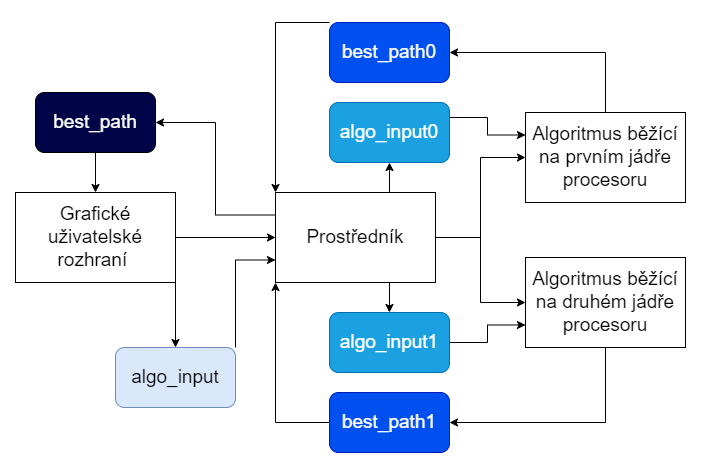
\includegraphics[width=15cm]{obrazky-figures/komunikace.png}
\caption{Komunikace aplikace}
\label{fig:komunikace ap}
\end{figure}
\chapter{Uživatelské rozhraní} 
\section{Informace o řešení a struktura GUI}
Grafické uživatelské rozhraní je implementováno pomocí modulu \textbf{Tkinter} v jazyce \textbf{Python}. K tomu, aby bylo grafické uživatelské rozhraní pro uživatele přívětivé a snadno použitelné, zvolil jsem jednoduchý a moderní design s pomocí knihovny \textbf{CustomTkinter}. Snažil jsem se také zvolit vhodné názvy pro jednotlivé popisky k prvkům, aby bylo jasné, co vlastně dělají. Dále jsem dodržoval konzistenci mezi jednotlivými prvky, včetně jejich stylu a chování, aby se zlepšila celková použitelnost grafického rozhraní a zabránilo se zmatení uživatele. Aplikace využívá chybové a informativní hlášky pro uživatele, aby byl uživatel informován, co dělá špatně. Grafické uživatelské rozhraní se skládá ze tří oken. Hlavní okno aplikace obsahuje plochu pro vygenerovaná místa a tlačítka pro ovládání nebo otvírání vedlejších oken. Další okno je určeno pro import míst z mapy, kde se nachází mapa a tlačítka pro ovládání. Poslední okno slouží k nastavení konkrétních algoritmů. Implementačně jsem jednotlivé okna rozdělil na třídy, každá v jiném souboru. Celý programový cyklus běží v hlavním okně a nepředává se nijak kontrola jiným oknům. Po skončení aplikace se, pro korektní ukončení aplikace, zjistí, jestli neběží jedno z vedlejších oken. Pokud vedlejší okno běží, tak se ukončí.


\section{Hlavní okno} \label{sec:main window}
Hlavní účel hlavního okna je zobrazení míst a cest mezi nimi. Plocha pro zobrazení míst se nachází uprostřed obrazovky na obrázku \ref{fig:main_window_basic}. Jednotlivé místa jsou reprezentovány bílými tečkami \ref{fig:main_window_dark_generated}, cesty mezi nimi pomocí černých čar \ref{fig:main_window_dark_solved}. 

\subsection{Widgety pro ovládání hlavního okna}
Nachází se v levé části programu, jak je vidět na kterémkoliv z obrázků \ref{fig:main_window_basic} \ref{fig:main_window_dark_generated} \ref{fig:main_window_dark_solved}. Zde je jejich seznam a k čemu slouží. 
\begin{itemize}
\item \textbf{Place generation mode} \textit{výběrové menu} -- Pro zvolení možnosti jakou chceme generovat místa náhodně, z souboru nebo z mapy.
\item \textbf{Algorithm types} \textit{výběrové menu} -- Pro zvolení jaký konkrétní algoritmus chceme použít pro řešení problému.
\item \textbf{Solve} \textit{tlačítko} -- Začne řešit problém obchodního cestujícího mezi vygenerovanými místy zvoleným algoritmem v \textbf{Algorithm types}.
\item \textbf{Stop} \textit{tlačítko} -- Přestane řešit problém obchodního cestujícího
nebo přestane generovat místa. Slouží k tomu, aby uživatel nemusel ukončovat aplikaci nebo čekat na vyřešení problému, pokud se rozhodl v průběhu, že ho vlastně nechce řešit, nebo zjistil, že by to trvalo příliš dlouho. Neslouží k zastavení a k následnému spuštění. Sice se po zmáčknutí tlačítka práce nesmaže. Ale to nastane až po dalším kliknutí na tlačítko \textbf{Generate} nebo \textbf{Solve}. 
\item \textbf{Clear roads} \textit{tlačítko} -- Slouží k smazaní cest mezi jednotlivými místy.
\item \textbf{Algorithm settings} \textit{tlačítko} -- Otevření nastavení zvoleného algoritmu v \textbf{Algorithm types}
\item \textbf{Appearance mode} \textit{výběrové menu} -- Slouží k přepínání mezi tmavým \ref{fig:main_window_dark_generated}  a světlým módem \ref{fig:main_window_basic}. 
\item \textbf{UI scaling} \textit{výběrové menu} -- Možnost měnit velikost widgetů od 80\% do 150\%
\end{itemize}


Dále se zde nacházejí widgety závisle na zvoleném \textbf{Place generation mode} Při zvolení možnosti \textbf{Random} \ref{fig:main_window_dark_generated}. Generujeme místa do plochy pseudonáhodně. A zobrazí se pouze následující widgety:
\begin{itemize}
\item \textbf{Number of places} \textit{textové pole} a \textit{posuvník} -- Textové pole určuje, kolik míst chceme vygenerovat, a je propojené s posuvníkem. Ten nabývá hodnot od 0 do 1000. Je zde možnost zadaní i větší hodnoty, a to ručním vepsáním hodnoty do textového pole. Pokud je špatný formát, například když tam napíšete nenumerický znak, vyskočí na vás chyba.
\item \textbf{Generate} \textit{tlačítko} - vygeneruje zvolený počet míst v textovém poli do modré plochy uprostřed obrazovky. 
\end{itemize}

Při zvolení možnosti \textbf{From Map} \ref{fig:main_window_basic} chceme použít reálnou mapu pro generování míst. A zobrazí se následující widgety. 
\begin{itemize}
\item \textbf{Add places} \textit{tlačítko} -- Přidá možnost přidat další místa k těm aktuálním. Spustí nové okno které složí k importu míst z reálné mapy, ale předchozí vygenerovaná místa se nesmažou. 
\item \textbf{Import places} \textit{tlačítko} -- Dělá úplně to samé jako tlačítko \textbf{Add places} s tím rozdílem, že se předchozí místa smažou.
\end{itemize}
Poslední možností je import souboru \textbf{From file} \ref{fig:main_window_dark_solved} v kterém jsou uložené místa a jejich souřadnice. Jak můžeme vidět na obrázku  Pro změnu se nám zobrazí zase: 
\begin{itemize}
\item \textbf{Select file} \textit{tlačítko} -- Po stisknutí tlačítka se zobrazí dialog pro výběr souboru. Zvolíme soubor s místy jejich souřadnicemi. A následně se nám zobrazí v modré ploše pro místa. 
\end{itemize}


\subsection{Pravidla pro používání tlačítek}
Pravidla pro používání tlačítek nejsou složité, ale asi by bylo dobré je zmínit. Pokud stisknete tlačítko \textbf{Generate} nebo \textbf{Solve} vytvoří se nové vlákno, kde běží generování míst nebo řešení algoritmu. To slouží k tomu, aby Tkinter aplikace nezamrzla. Další věc, která nastane po stisknutí tlačítek je, že se nastaví flag, který říká, že něco běží na pozadí na True. Následně pokud chceme zase stisknut některé z tlačítek, nebude nám to umožněno, dokud se aktuální činnost nedokončí. Poté se flag nastaví zpět na False. 

\subsection{Vyskakovací informativní a chybové hlášky}
Existují celkem 4 informativní a 1 chybová hláška.Příklad chybové hlášky 

\textbf{Informativní} \ref{fig:main_window_info} jsou:
\begin{itemize}
    \item \textbf{You didn´t generate places before running the solution}
    
        - Hláška se vás snaží upozornit na to, že jste chtěl zapnout řešení algoritmu předtím než jste vygeneroval nějakým způsobem místa. Proto aby se vám nezobrazovala můžete například náhodně vygenerovat místa nebo je nahrát ze souboru, či z mapy.  
    \item \textbf{You can´t start new solve while still solving}
    
        - Tato hláška vás upozorňuje na to, že jste se pokusil nové řešení když už nějaké probíhá. Proto aby se vám nezobrazovala musíte počkat na to než se dokončí aktuální řešení. A teprvé spustit nové. 
    \item \textbf{You can´t generate new places while still solving}
    
        - Tato hláška je velmi podobná té předchozí s tím rozdílem, že se snažíte vygenerovat nové místa, když stále probíhá řešení aktuálního problému. A zase musíte počkat k dokončení aktuálního problému před generováním nových míst. 
    \item \textbf{Distance: [distance] Count of visisted places: [count of visited places]}
    
        - Poslední z informativních hlášek vám po dokončení řešení problému obchodního cestujícího vypíše celkovou vzdálenost, která se zobrazí i v dolní části uprostřed obrazovky. Ještě zobrazí počet míst, které navštívil. 
\end{itemize}
\textbf{Chybová} \ref{fig:main_window_error} je:
\begin{itemize}
    \item \textbf{Wrong format of places count Right format is [int] > 1}
        - Hláška se vás snaží upozornit, že nemůžete vygenerovat místa, jelikož jste do textového pole pod \textbf{Number of places} zadal hodnotu, která není číslo, které jde převést na číslo typu integer. Nebo je číslo menší jak 2 v tom případě nemá smysl problém obchodního cestujícího pro tolik míst ani řešit. 
\end{itemize}




\begin{figure}
    \centering
    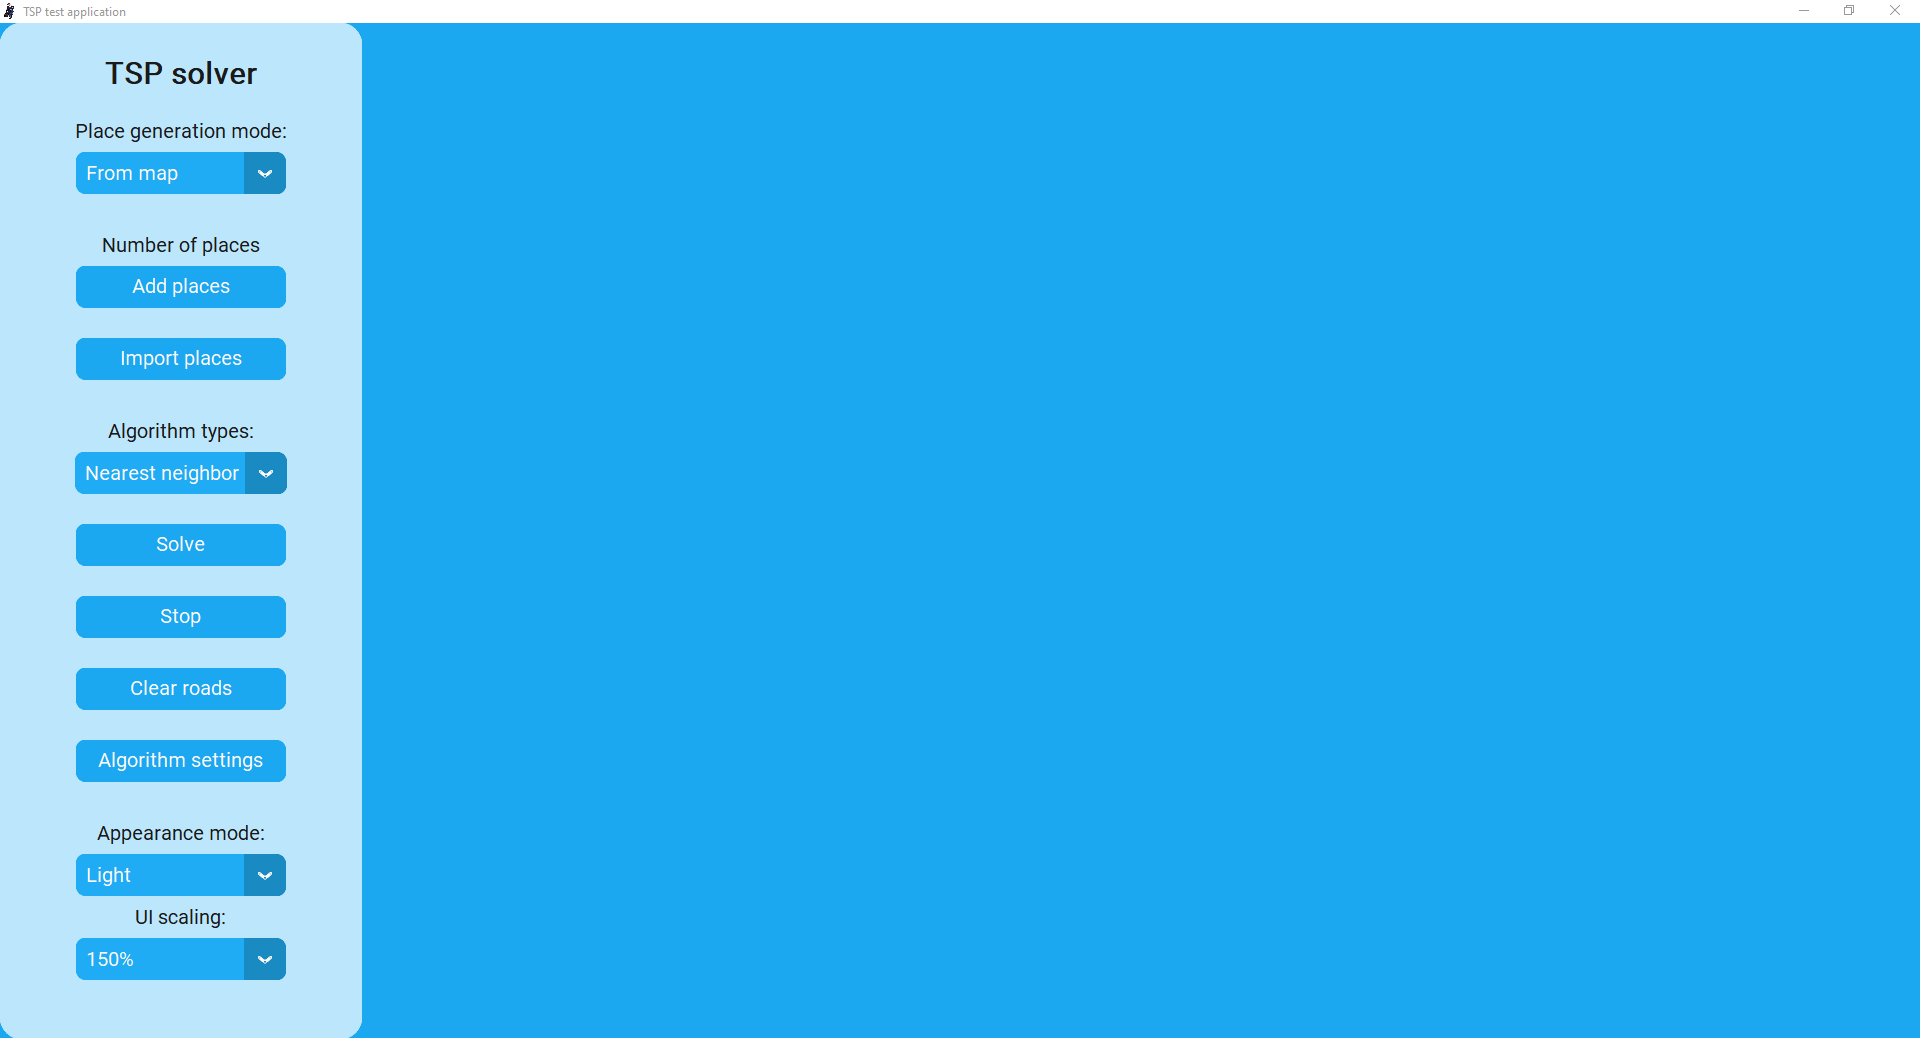
\includegraphics[width=15cm]{obrazky-figures/main_window.png}
    \caption{Hlavní okno aplikace}
    \label{fig:main_window_basic}
\end{figure}
\begin{figure}
    \centering
    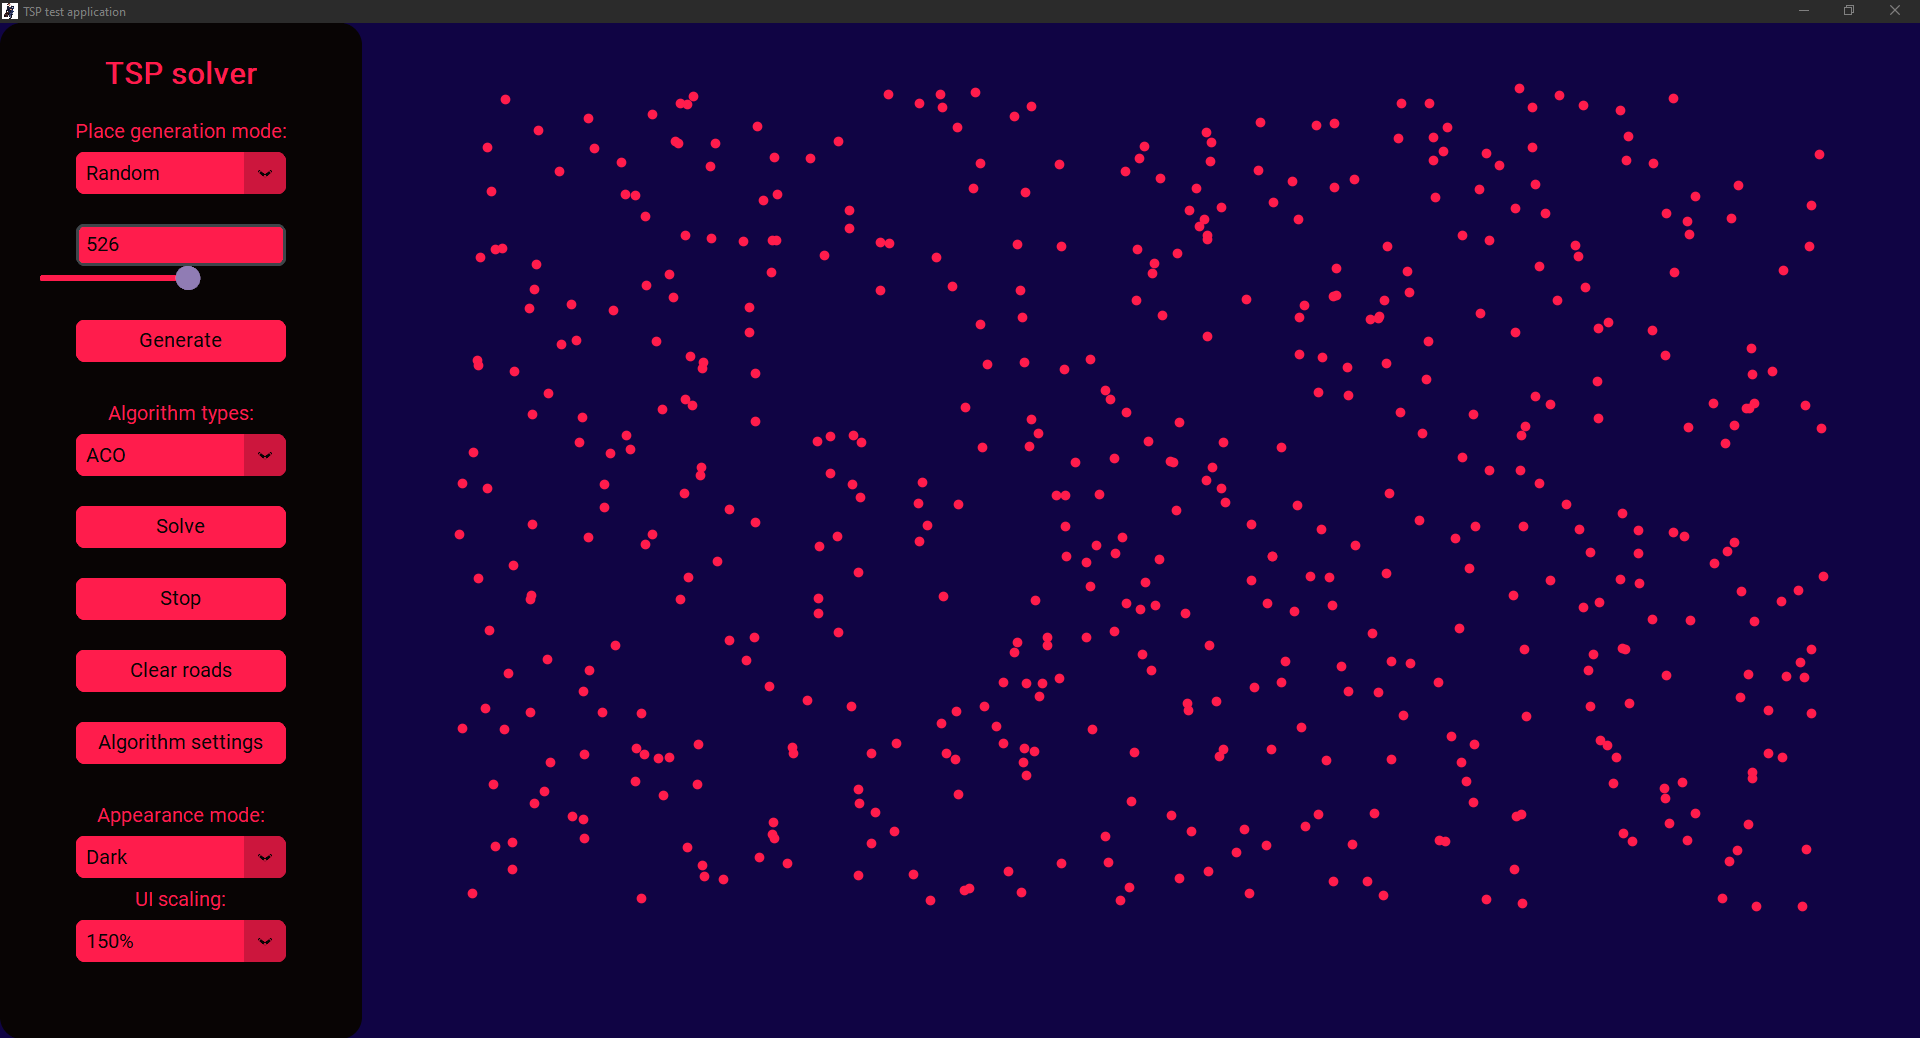
\includegraphics[width=15cm]{obrazky-figures/main_window_random_places_dark.png}
    \caption{Hlavní okno aplikace dark mode a vygenerované místa}
    \label{fig:main_window_dark_generated}
\end{figure}
\begin{figure}
    \centering
    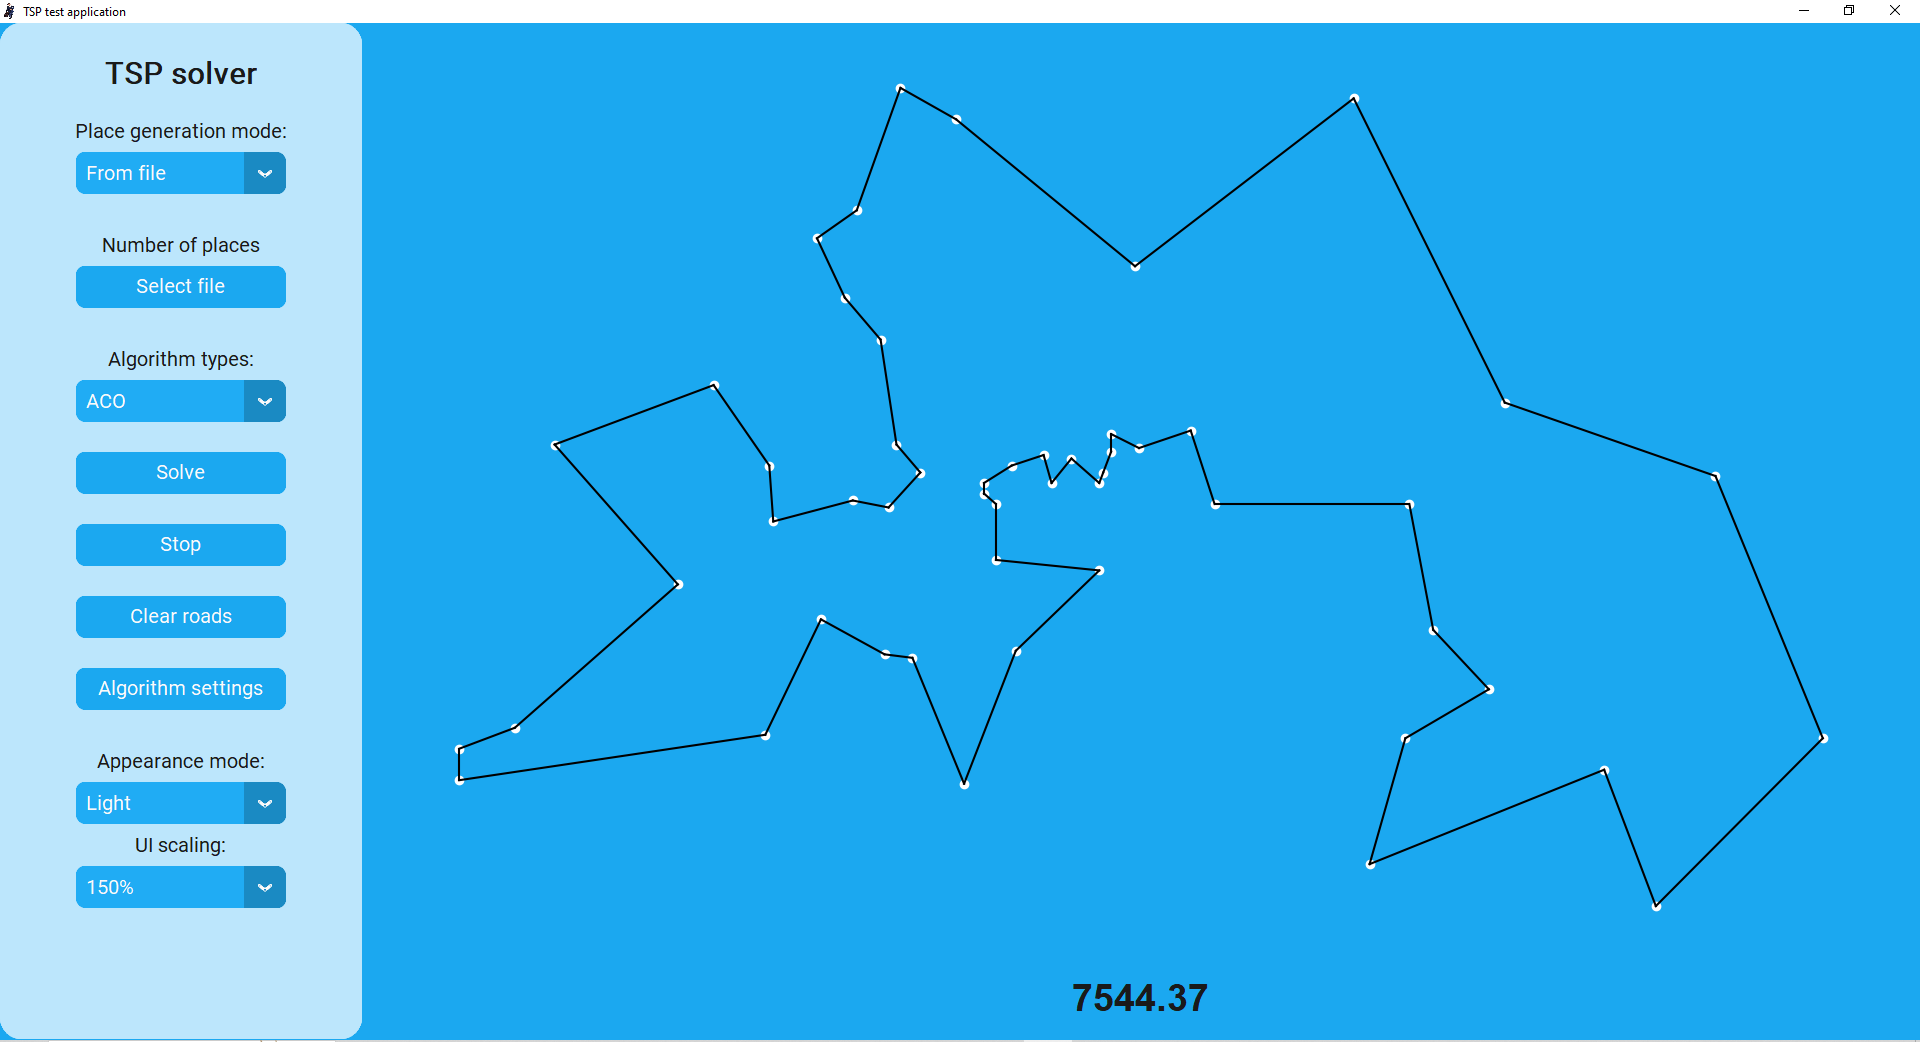
\includegraphics[width=15cm]{obrazky-figures/main_window_solved_from_file.png}
    \caption{Hlavní okno aplikace s vyřešeným problémem obchodního cestujícího(berlin52)}
    \label{fig:main_window_dark_solved}
\end{figure}
\begin{figure}
    \centering
    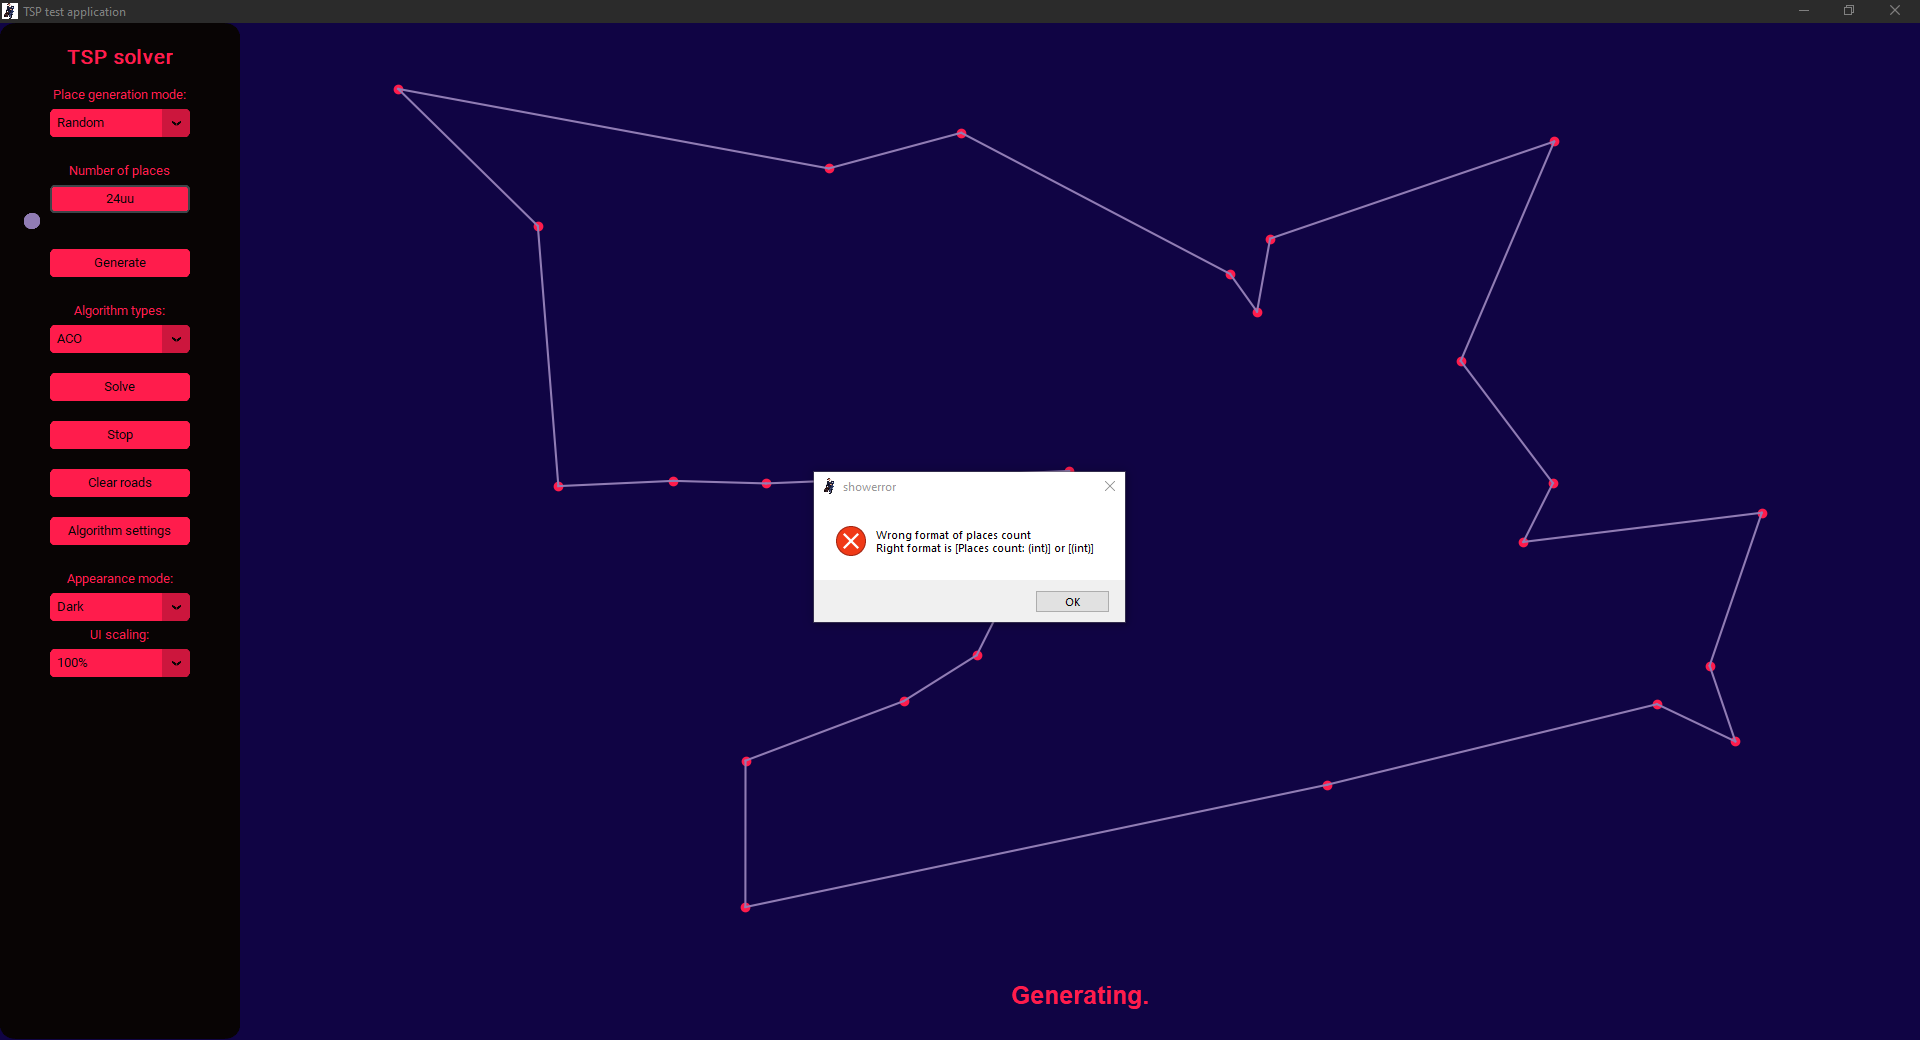
\includegraphics[width=15cm]{obrazky-figures/main_window_error.png}
    \caption{Chybová vyskakovací hláška}
    \label{fig:main_window_error}
\end{figure}
\begin{figure}
    \centering
    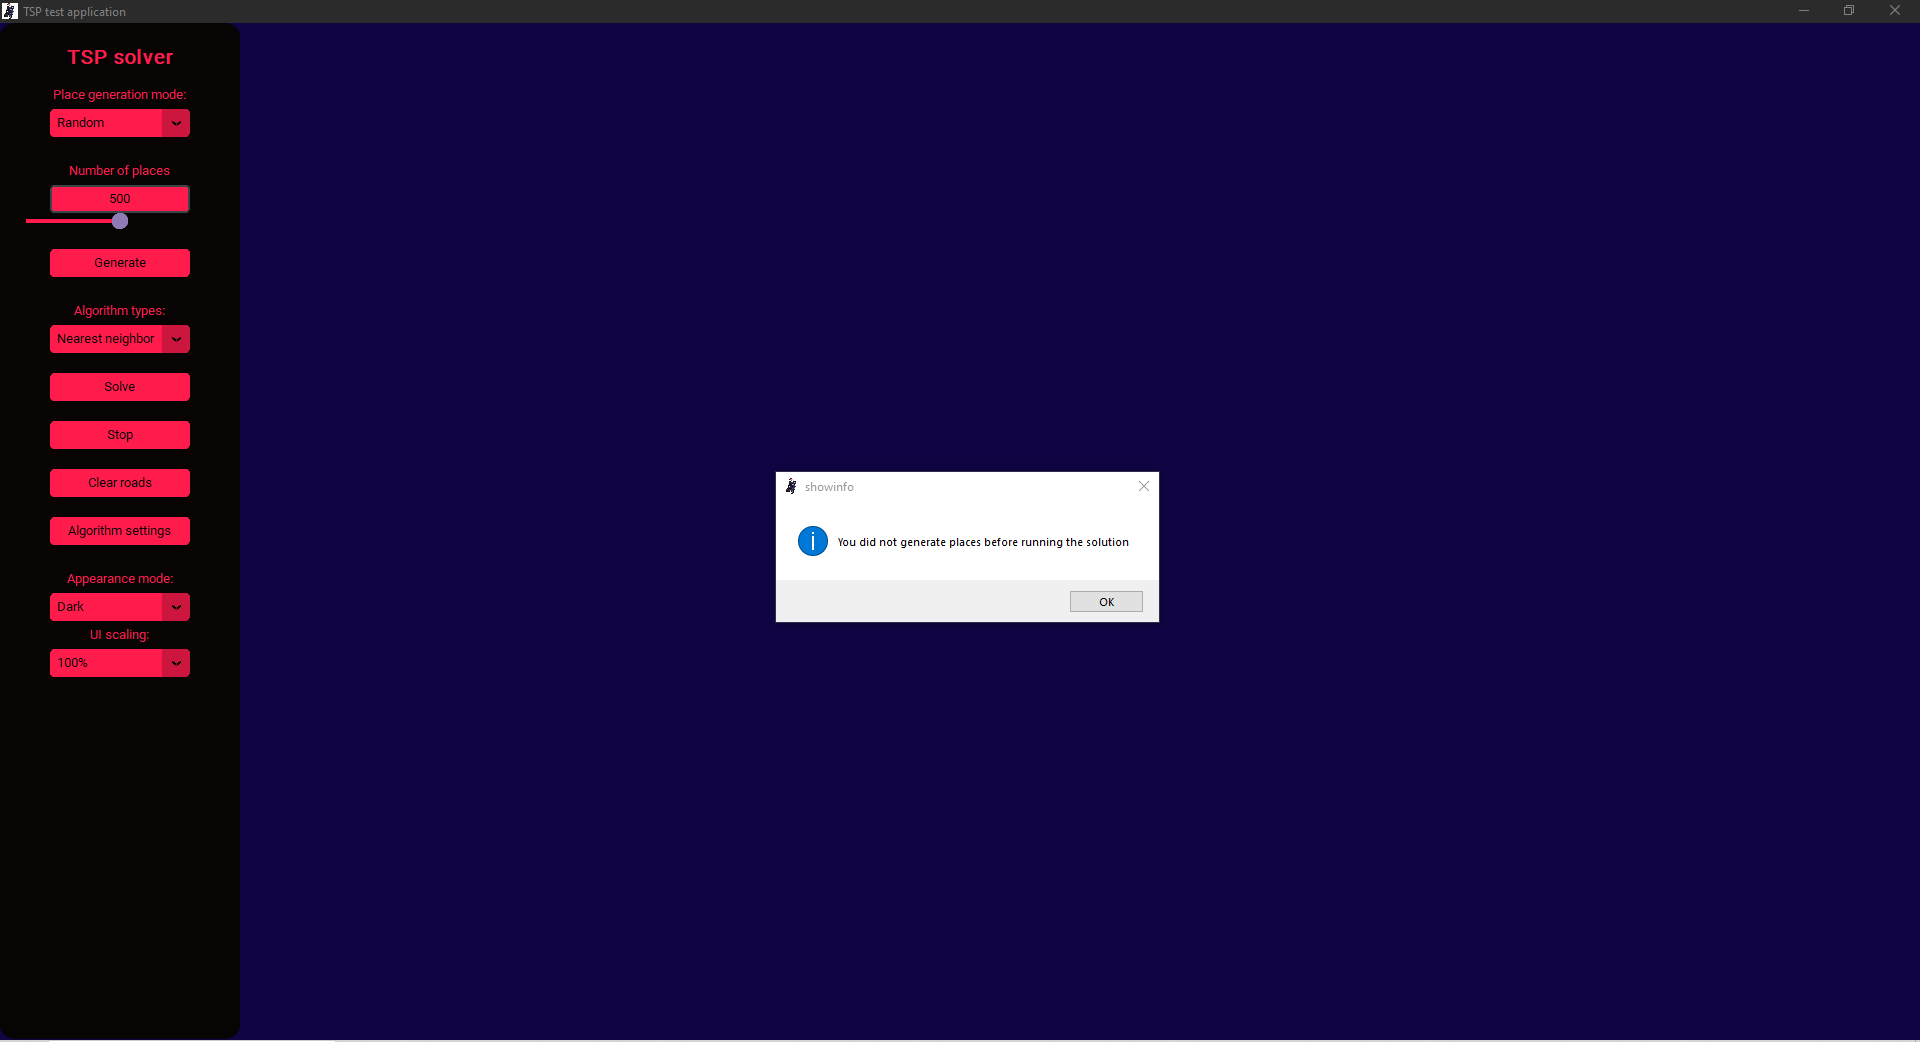
\includegraphics[width=15cm]{obrazky-figures/main_window_info_no_places.png}
    \caption{Informativní vyskakovací hláška}
    \label{fig:main_window_info}
\end{figure}



\newpage
\section{Okno pro import míst z mapy}
Další okno aplikace do kterého se můžete dostat slouží k importu míst z reálné mapy. Implementačně jsem to zpracoval pomocí knihovny od stejného autora jako \textbf{CustomTkinter}, takže zde není nějaké problematické spojení těchto dvou knihoven dohromady. Dokonce jsou na githubu konkrétní příklady spojení těchto knihoven dohromady\cite{TkinterMapView}. Autorem je Tom Schimansky. Obrazovku pro import míst z mapy můžeme vidět na obrázku \ref{fig:map_window}. 
\subsection{Ovládání}
Po levé straně se nacházejí \textbf{widgety} pro ovládání. Zde je jejich seznam:
\begin{itemize}
    \item \textbf{Remove last marker} \textit{tlačítko} -- Smaže poslední značku tu s největším číslem. 
    \item \textbf{Remove all marks} \textit{tlačítko} -- Smaže všechny značky, pokud nějaké jsou. 
    \item \textbf{Import marks} \textit{tlačítko} -- Zavře okno a nahraje značky, které jsme zvolili do hlavního okna.
    \item \textbf{Tile server} \textit{výběrové menu} -- Slouží k tomu jaký server pro mapy chceme použít celkově to mění design mapy. 
\end{itemize}
Celkové ovládání mapy je velmi jednoduché a intuitivní. Kliknutím levého tlačítka myši kam chceme, se objeví značka, tj. místo, které chceme nahrát do hlavní obrazovky. Obrazovku můžeme posunout pomocí stisknutí levého tlačítka a hýbání s ní. Pokud chceme přiblížit nebo oddálit, slouží nám + a - v levé horní části obrazovky či kolečko na myši.

\subsection{Z mapy do hlavního okna}

Jak jsem již zmínil, po stisknutí tlačítka \textbf{Import marks} se jednotlivé značky nahrají do hlavního okna. Aby to fungovalo, musejí se udělat dvě důležité věci. První je spočítání vzdálenosti mezi dvěma místy na planetě. Konkrétně používám funkci \textbf{distance.geodesic} z knihovny geopy\cite{GeopyDistance}. Jelikož Země není koule, ale geoid, funkce využívá \textbf{Vincentyho formuli}. Původně jsem si myslel, že použiji Haversinovu formuli, která počítá vzdálenost dvou bodů na sféře. Vzorec Vincentyho formule je docela složitý a nemá s projektem moc společného, tak ho tady nebudu uvádět, ale můžete ho najít například na \cite{VincentyFormulae}.

Druhou důležitou věcí je celková normalizace, jelikož plocha která zobrazuje místa je v rozsahu 0-1 pro x i pro y. Je to kvůli tomu, aby se nemusela pro nové místa plocha zbytečně mazat. Vzorec pro normalizaci je následovný \cite{SENormalizationAns}. Předpokládejme, že x je list prvků $x_i$.
\begin{equation*}
    \scalebox{1.2}{$normalized\_x_i=\frac{x_i-\min (x)}{\max (x)-\min (x)}$}
\end{equation*}
Já využívám souřadnice x i y proto jsem provedl následující úpravy:

    \begin{equation*}
    \scalebox{1.2}{$xdiv = \max (x)-\min (x)$}
    \end{equation*}
    \begin{equation*}
    \scalebox{1.2}{$ydiv = \max (y)-\min (y)$}
    \end{equation*}
    \begin{equation*}
    \scalebox{1.2}{div = xdiv if xdiv > ydiv else ydiv}
    \end{equation*}
    \begin{equation*}
    \scalebox{1.2}{$normalized\_x_i=\frac{x_i-\min (x)}{div}$}
    \end{equation*}
    \begin{equation*}
    \scalebox{1.2}{$normalized\_y_i=\frac{y_i-\min (y)}{div}$}
    \end{equation*}

Celkově to slouží k tomu, aby se zachoval poměr mezi x a y souřadnicemi na mapě. Pokud bychom zvolili dvě místa v libovolném poměru, vždy bude jedno místo v levém horním rohu a druhé v pravém dolním rohu, což platí, pokud pro x a y využijeme první vzorec. Druhý vzorec tomu zabraňuje tím, že dělitel je vždy stejný pro x i y. Samozřejmě se zde uchovává i poměr mezi x a y souřadnicemi, ale jelikož Země není plochá, ale má geoidový tvar, nebude to zcela přesné, ale slouží to pouze k zobrazení míst. Máme již vypočítané celkové vzdálenosti celkem přesně, takže to není velký problém.

Na obrázku \ref{fig:map_window} vidíme, že jsme zvolili celkem 15 míst, a to jsou některé školy v Brně, ale ne všechny. Abychom mohli vypočítat nejlepší cestu mezi nimi, musíme stisknout tlačítko pro \textbf{Import marks}. Následně se okno pro mapu vypne a na hlavním okně se zobrazí místa na ploše podobně jako na obrázku \ref{fig:normalized}, s tím rozdílem, že tam ještě nebudou černé čáry mezi místy. Vybereme algoritmus, jakým chceme problém řešit, a klikneme na tlačítko \textbf{Solve}. Poté bude hlavní okno vypadat přesně jako na obrázku \ref{fig:normalized}. V dolní části obrazovky se zobrazí celková vzdálenost mezi všemi místy, která je 23.5588. Černé čáry mezi místy značí cesty mezi nimi. Toto je nejkratší možná cesta, kterou algoritmus našel.


\begin{figure}[H]
    \centering
    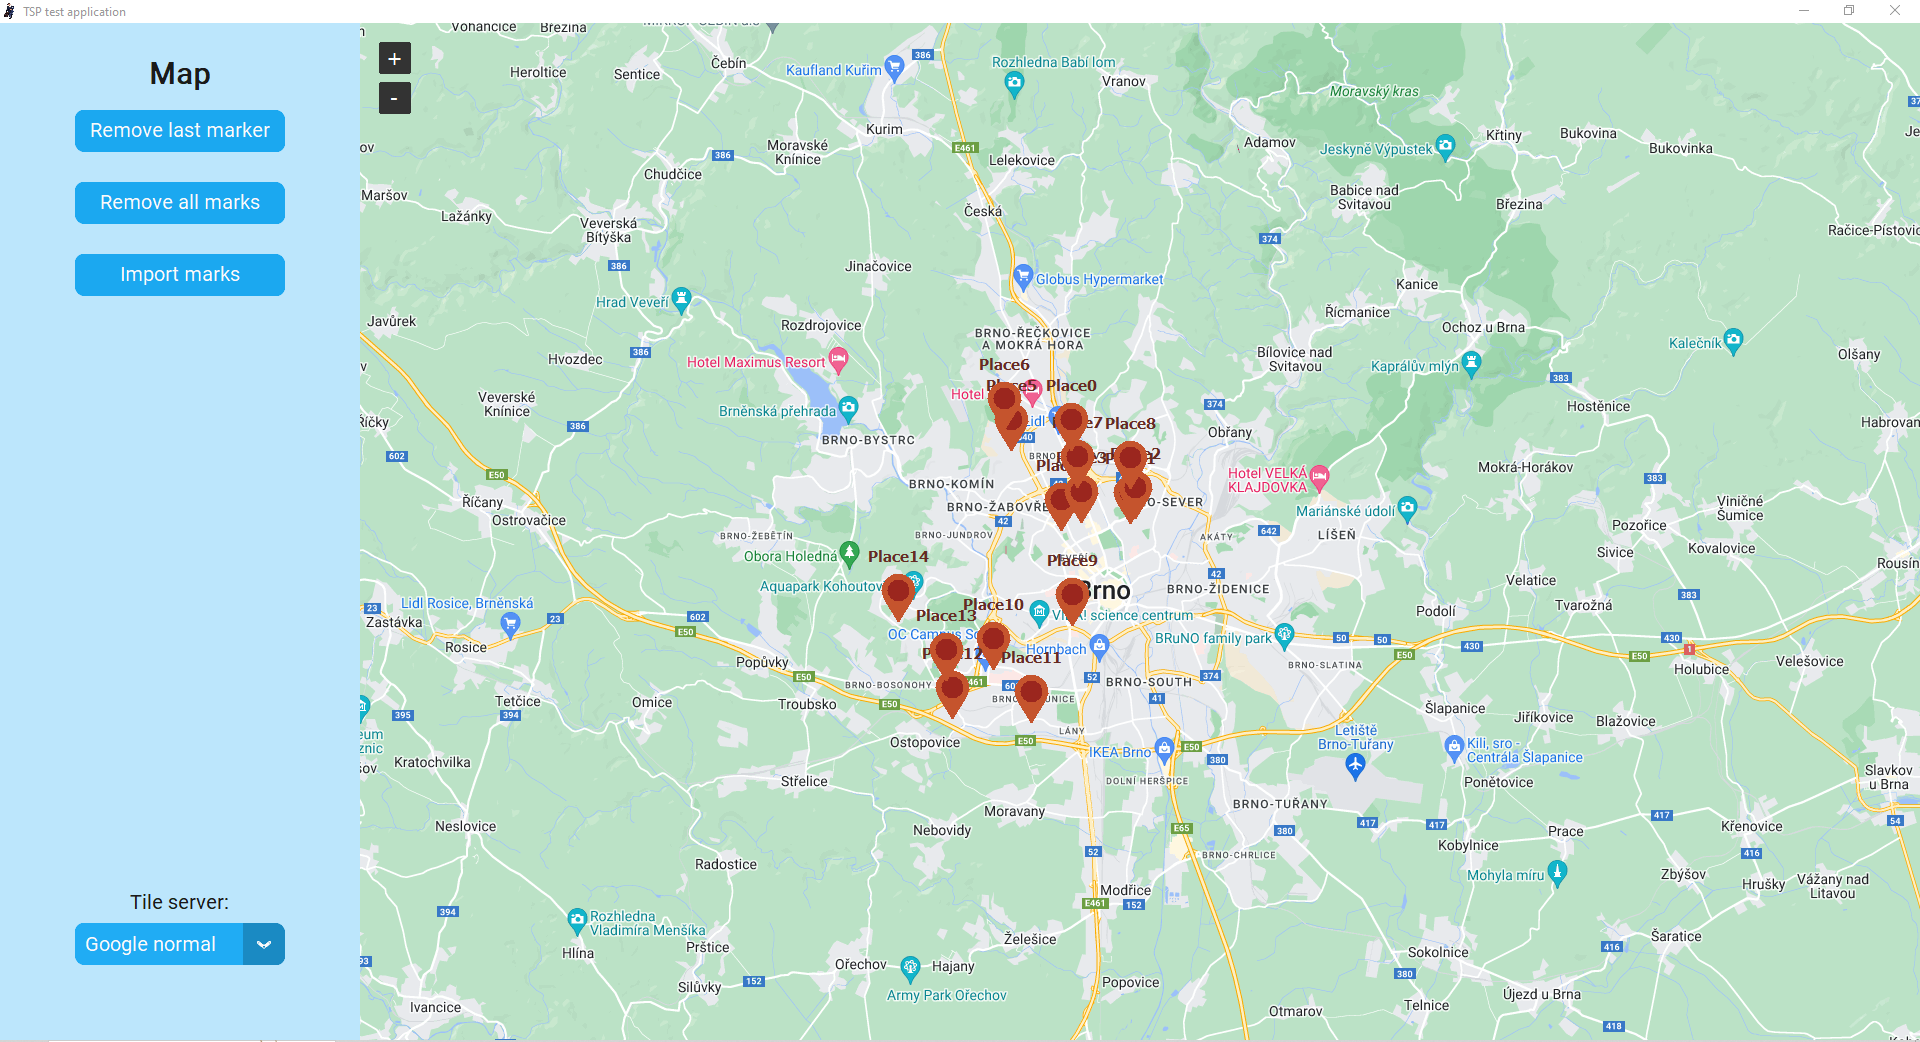
\includegraphics[width=15cm]{obrazky-figures/map_window_marks.png}
    \caption{Okno pro import míst z mapy s značkami}
    \label{fig:map_window}
\end{figure}
\begin{figure}[H]
    \centering
    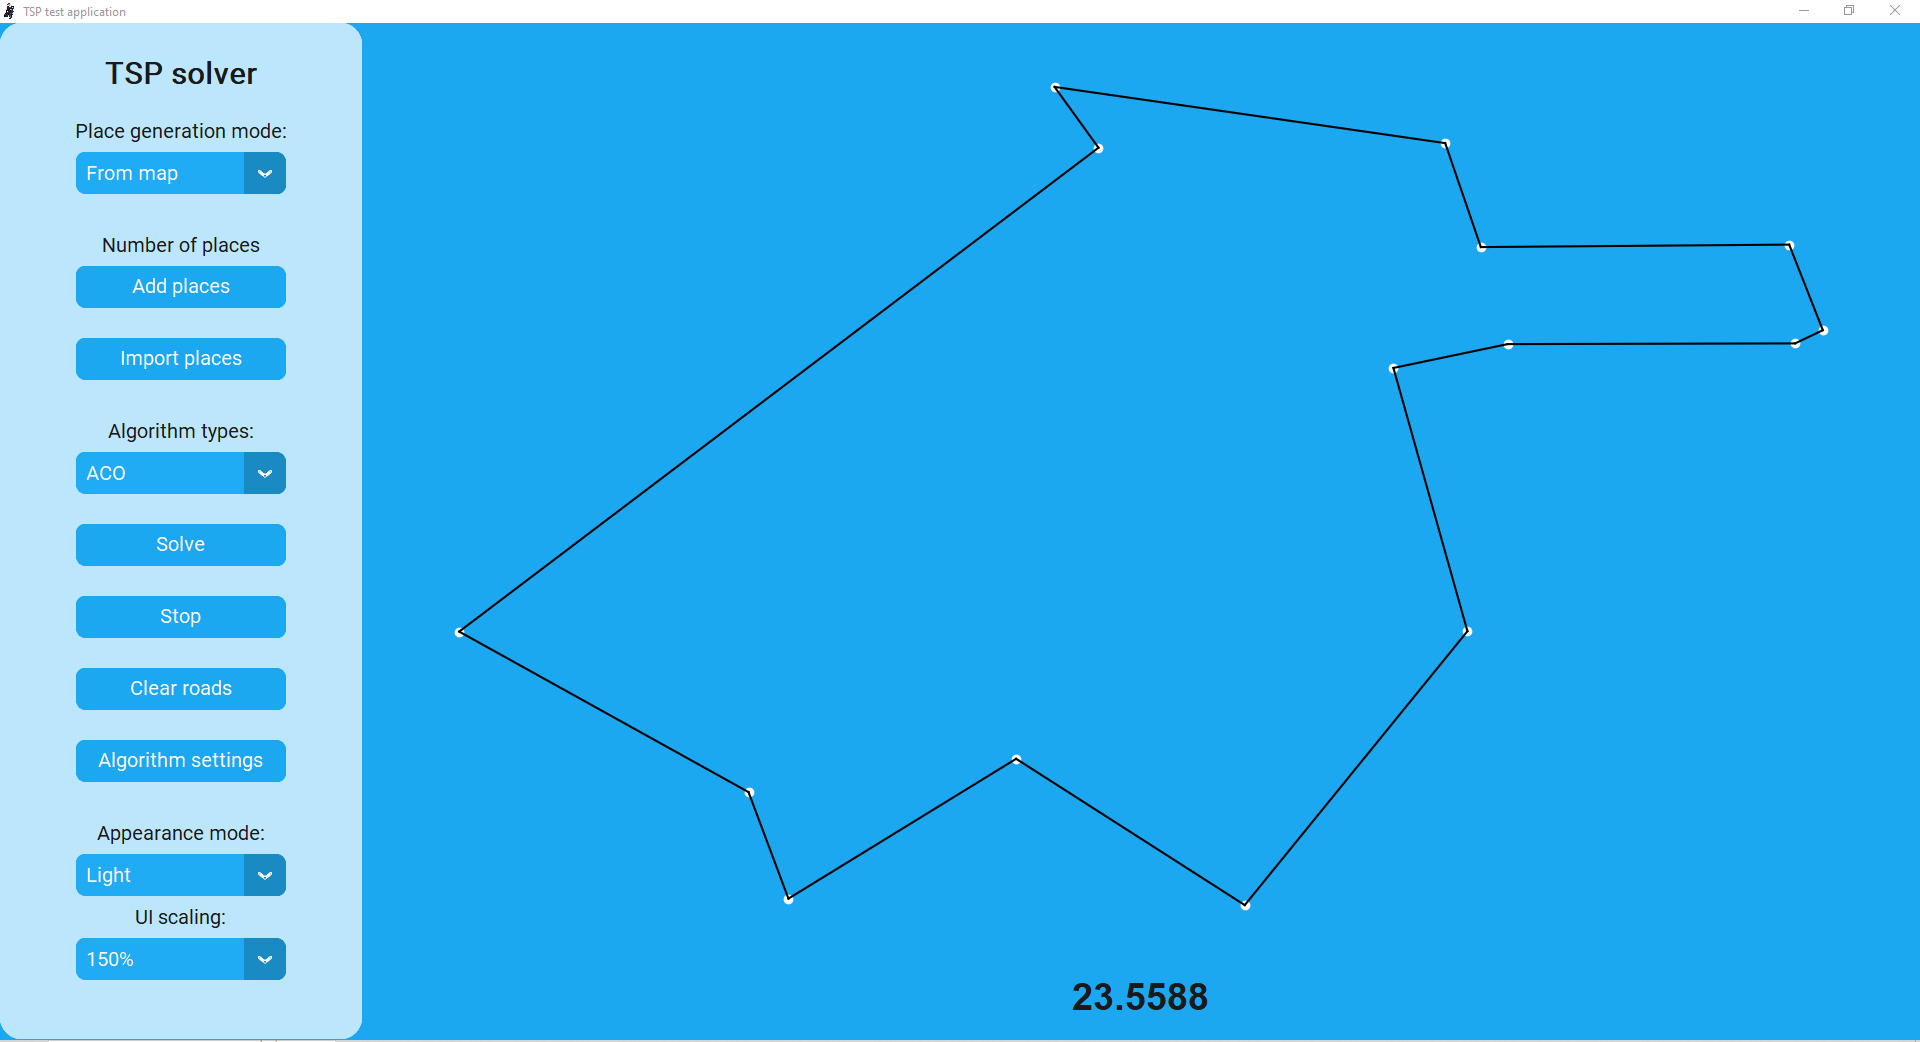
\includegraphics[width=15cm]{obrazky-figures/normalized_solved.png}
    \caption{Hlavní okno s nahranými značkami z mapy}
    \label{fig:normalized}
\end{figure}

\section{Okno pro nastavení Ant Colony Optimization}
První okno sloužící pro nastavení konkrétně pro Ant Colony Optimization je na obrázku \ref{fig:settings_ACO}. Okno je velmi jednoduché pouze název parametru, který můžete měnit a textové pole, pro jeho zadání. Hodnoty už jsou přednastavené. Pokud najedete na nějaké textové pole zobrazí se vám informace z jakého rozsahu je můžete vybírat a jaký by měl být optimální. Okno kontroluje pouze typ čísla int či float a ne rozsah. A jestli je není číslo menší než 0. Ale nekontroluje se, jestli zadáte například víc jader než máte. Předpokládám, že v tom případě by to Python script pro paralerní spouštění na více jádrech. Nespustil paralérně, ale vždy by čekal na uvolnění některého z jader. Silně nedoporučuji využívat všechny jádra zvlášť pro velké problémy a ještě v kombinaci s moc agenty tedy vlákny. Může se stát, že váš počítač bude neovladatelný, kvůli vytížení procesoru. Může se to jevit jako problém, ale já v tom problém nevidím, jelikož uživatel aplikace by měl zvážit co by mělo být pro jeho problém optimální nastavení. Osobně doporučuji využívat u větších problémů 500 míst a víc. okolo 25\% jader procesoru a okolo 50 agentů. Pro menší problémy do 50 míst můžete využít klidně všechny jádra procesoru a 100 agentů.
\subsection{Jednotlivé parametry v nastavení}
Popíši zde pouze pravou část nastavení, jelikož k levé části je už víc v \ref{sec:params}
\begin{itemize}
    \item \textbf{Iterations} \textit{int} -- Počet iterací ACO algoritmu, pouze pro jednoho agenta. Počet iterací musí být větší jak 0. A optimální je tak od 100 iterací do 1000 iterací, hodně záleži na počtu agentů. Všiml jsem si, že od nějakého počtu iterací ACO už lepší cestu najde jen velmi nepravděpodobně. Celkový počet iterací algoritmu je roven vztahu:
    \begin{center}
    \scalebox{1.2}{Count of agents $*$ Number of cores $*$ Iterations}
     \end{center}
     
    \item \textbf{Count of agents} \textit{int} -- Počet agentů(vláken) nebo chcete-li mravenců. Kteří procházejí každý svými iteracemi a aktualizují globální feromony společné pro všechny mravence. Počet agentů by měl být větší než 0, což je samozřejmé. Doporučuji tak od 5 agentů do 100 agentů, zase záleží na počtu iterací počtu využitých jader a velikosti problému. 
    \item \textbf{NN iterations multiplayer} \textit{float} -- Tento parametr slouží k vynásobení celkového počtu míst tímto parametrem a získání z toho počet iterací Nearest Neighbor Algorithm. Pro nastavení prvotních hodnot $\tau$. Ideální hodnota je tak okolo 1, ale reálně nastavení $\tau$ pomocí Nearest Neighbor Algorithm nebude mít velký vliv na řešení problému. Jediné k čemu slouží je, aby bylo prvotní cesta lepší než čistě přes ACO, tím se sníží počet iterací. Zde je vzorec: 
    \begin{center}
    \scalebox{1.2}{Počet iterací NN = NN iterations multiplayer $*$ Počet míst }
     \end{center}
        
    \item \textbf{NN lenght of path} \textit{int} -- Tento parametr taky slouží k prvotnímu nastavení $\tau$. Je to celková délka cesty. Měl by být větší jak 0, ale pokud nastavíte 0, tak se Nearest Neighbor Algorithm prostě nepoužije. Není dobré ani nastavovat moc velkou délku cestu. Protože algoritmus už bude mít všechny výhodné místa spojené tím pádem připadnou méně atraktivní cesty. Ideální je tak okolo 2. Když si to zkusíte představit většinou to budou cesty, které se budou využívat pro optimální řešení samozřejmě ne vždy. 
    \item \textbf{Number of cores} \textit{int} -- Zde se určuje počet jader, na kterých bude algoritmus spuštěn nezávisle na ostatních. Popis jak funguje komunikace a vybírání cesty je detailněji popsaný už v \ref{sec:comunication}.
\end{itemize}


\begin{figure}
    \centering
    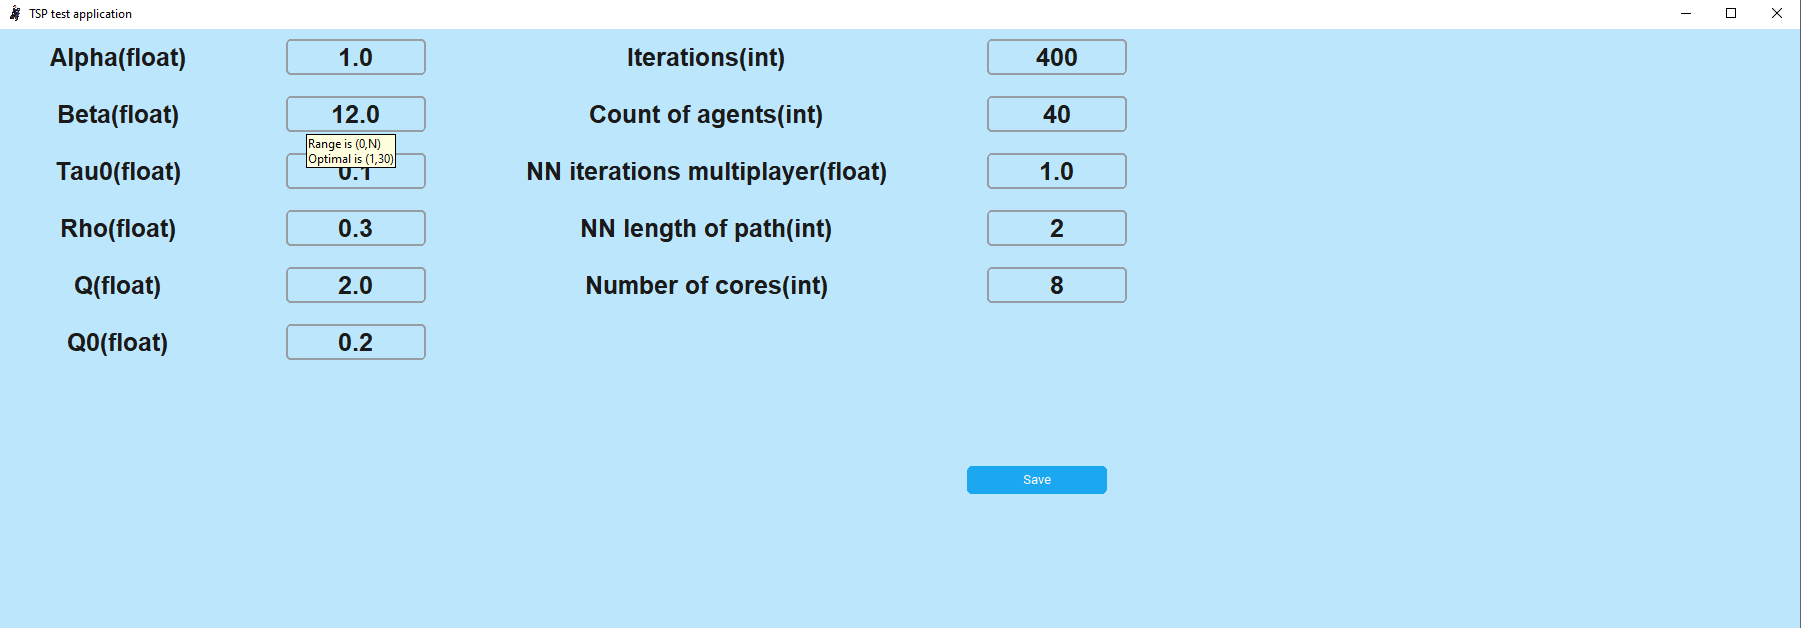
\includegraphics[width=15cm]{obrazky-figures/ACO_settings.png}
    \caption{Okno pro nastavení Ant Colony Optimization}
    \label{fig:settings_ACO}
\end{figure}


\section{Okno pro nastavení mého algoritmu}
Toto další okno slouží k nastavení mých algoritmů. Abyste se k němu dostali, stačí změnit \textbf{Algorithm types} na \textbf{MyAlgo}. Provádí jednoduché kontroly, zda jsou zadaná čísla typu celého čísla větší než 0. Dále zde naleznete 2 přepínače.

\subsection{Jednotlivé parametry v nastavení}
\begin{itemize}
    \item \textbf{Start NN size} -- Jedná se o velikost, do které se mohou přidávat sousedící prvky, s kterými se tvoří lepší řešení pomocí 2-opt algoritmu.
    \item \textbf{Middle NN size} -- Jedná se o střední velikost, do které se mohou přidávat sousedící prvky, s kterými se tvoří lepší řešení pomocí 2-opt algoritmu.
    \item \textbf{Last NN size} -- Jedná se o poslední velikost, do které se mohou přidávat sousedící prvky, s kterými se tvoří lepší řešení pomocí 2-opt algoritmu.
    \item \textbf{Start NN count} -- Počet prvotně vygenerovaných řešení, na které nebyla aplikována \textbf{Last NN size}, a vybírá se vždy nejlepší z nich.
    \item \textbf{Rounding} -- Zaokrouhlování vzdáleností, které používají lidé s kterými jsem porovnával výsledky. Nejspíš kvůli tomu, aby nemuseli vzdálenosti ukládat, jako desetinné číslo, ale jako celé číslo. 
    \item \textbf{Segments} -- Použití optimalizace tím, že se řešení rozdělí na segmenty a v nich se náhodně generuje řešení a aplikovává se stejný postup, jako u normálního řešení. Tímto se snažíme segmenty zlepšit. 
\end{itemize}





\chapter{Testování} Testování jsem prováděl na počítači s 64bitovým operačním systémem Windows 10 Education. S procesorem AMD Ryzen 7 3750H with Radeon Vega Mobile Gfx 2.30 GHz a 5,93 GB RAM paměti. Do 1500 míst jsou testovány oba algoritmy od 1500 míst, jelikož ACO začíná být neefektivní a ne tak účinné jako můj algoritmu, provádím testy pouze mého algoritmu. \textbf{Potom co jsem provedl většinu testů jsem si uvědomil, že nepoužívají vzdálenost typu double, ale int, což mi reálně zhoršilo výsledky}. Nepřepsal jsem algoritmus k tomu, aby pracoval s inty i když by to určitě urychlilo výpočet, ale bylo by zde problematické pracování s náhodně generovanými místy, jelikož ty jsou jen v 0-1 rozsahu. Pouze je možnost zapnout zaokrouhlování. \textbf{Zaokrouhlování je potřeba zapnout před generováním míst tedy počítání vzdáleností mezi nimi} . Pro některé sady to bude mít minimální vliv, protože například, jestli bude vzdálenost 400000 nebo 400001 je irelevantní změna a výslednou cestu to nijak nezmění. Sady na, které ovšem tato skutečnost bude mít vliv jsou místa generovaná uměle, jelikož jejich vzdálenosti jsou o dost menší než ty z reálných map.  
\section{Popis tabulky mého algoritmu}
\begin{itemize}
    \item \textbf{Délka cesty} -- Délka nejlepší cesty, kterou algoritmus našel. 
    \item \textbf{Doba běhu} -- Doba běhu algoritmu i s načítáním míst z souboru a zápisem nejlepší cesty do souboru. 
    \item \textbf{Bez souboru} -- Doba běhu algoritmu s už načtenými místy a bez zápisu nejlepší cesty do souboru. 
    \item \textbf{Chybovost} -- Procentuální chyba řešení.
    \item \textbf{SNN} -- Počáteční počet sousedů v nastavení je reprezentovaná jako \textit{Start NN size}.
    \item \textbf{MNN} -- Střední počet sousedů v nastavení je reprezentovaná jako \textit{Middle NN size}.
    \item \textbf{LNN} -- Poslední počet sousedů v nastavení je reprezentovaná jako \textit{Last NN size}.
    \item \textbf{SC} -- Počet prvotních řešení v nastavení je reprezentovaná jako \textit{Start NN count}.
    \item \textbf{Segmenty} -- Využití rozdělení na segmenty pro zlepšení řešení.
\end{itemize}

\section{Popis tabulky ACO}
    \begin{itemize}
    \item \textbf{Délka cesty} -- Délka nejlepší cesty, kterou algoritmus našel. 
    \item \textbf{Doba běhu} -- Doba běhu algoritmu i s načítáním míst z souboru a zápisem nejlepší cesty do souboru.  
    \item \textbf{Chybovost} -- Procentuální chyba řešení.
    \item \textbf{$\alpha$} -- Reprezentuje důležitost vyloučeného feromonu na cestě.
    \item \textbf{$\beta$} -- Reprezentuje faktor viditelnosti na cestě.
    \item \textbf{$\rho$} -- Koeficient odpařování feromonu. 
    \item \textbf{Q} -- Intenzita feromonu, kterou představuje celkový feromon. 
    \item \textbf{Q0} -- Vyjadřuje s jakou pravděpodobností se zvolí nejlepší cesta podle aktuálního $\tau$.
    \item \textbf{Ag} -- Počet agentů.
    \item \textbf{It} -- Celkový počet iterací 
    \item \textbf{C} -- Počet jader na kterých algoritmus běží. 
\end{itemize}



\section{Testovací sada berlin52}
Pro testovací sadu s 52 místy berlin52 se oběma algoritmům povedlo nalézt optimální řešení. Které je dlouhé \textbf{7544.37}. Snímek optimálního řešení nalezeno oběma algoritmy je k dispozici: \ref{fig:berlin52}.  

\begin{table}[H]
\caption{berlin52-ACO}
\resizebox{\columnwidth}{!}{%
\begin{tabular}{|l|l|l|l|l|l|l|l|l|l|l|}
\hline
\textbf{Délka cesty} & \textbf{Doba běhu} & \textbf{Chybovost} & \cellcolor[HTML]{FFFFFF}{\color[HTML]{202124} \textbf{$\alpha$}} & \cellcolor[HTML]{FFFFFF}{\color[HTML]{202124} \textbf{$\beta$}} & \cellcolor[HTML]{FFFFFF}{\color[HTML]{202124} \textbf{$\rho$}} & \textbf{Q} & \textbf{Q0} & \textbf{Ag} & \textbf{It} & \textbf{C} \\ \hline
7544.37 & 6s & 0\%      & 1 & 3  & 0.1 & 200000 & 0.1 & 150 & 50  & 4 \\ \hline
7826.0  & 6s & 3.733\%  & 1 & 3  & 0.1 & 200000 & 0.1 & 20  & 20  & 4 \\ \hline
7658    & 6s & 1.5062\% & 1 & 3  & 0.1 & 200000 & 0.1 & 20  & 100 & 4 \\ \hline
7606.95 & 6s & 0.8295\% & 1 & 13 & 0.1 & 200000 & 0.1 & 150 & 50  & 4 \\ \hline
\end{tabular}%
}
\end{table}

\begin{table}[H]
\caption{berlin52-MyAlgo}
\resizebox{\columnwidth}{!}{%
\begin{tabular}{|l|l|l|l|l|l|l|l|l|}
\hline
\textbf{Délka cesty} & \textbf{Doba běhu} & \textbf{Bez souboru} & \textbf{Chybovost} & \textbf{SNN} & \textbf{MNN} & \textbf{LNN} & \textbf{SC} & \textbf{Segmenty} \\ \hline
7544.37              & 6s                 & 23ms                 & 0\%                & 1            & 12           & 33           & 4           & Ne                \\ \hline
7544.37              & 6s                 & 14ms                 & 0\%                & 1            & 12           & 33           & 1           & Ne                \\ \hline
7544.37              & 6s                 & 3ms                  & 0\%                & 1            & 4            & 11           & 1           & Ne                \\ \hline
7716.69              & 6s                 & 3ms                  & 2.2841\%           & 5            & 6            & 11           & 1           & Ne                \\ \hline
7544.37              & 6s                 & 2ms                  & 0\%                & 1            & 2            & 3            & 1           & Ne                \\ \hline
\end{tabular}%
}
\end{table}
\begin{figure}[H]
    \centering
    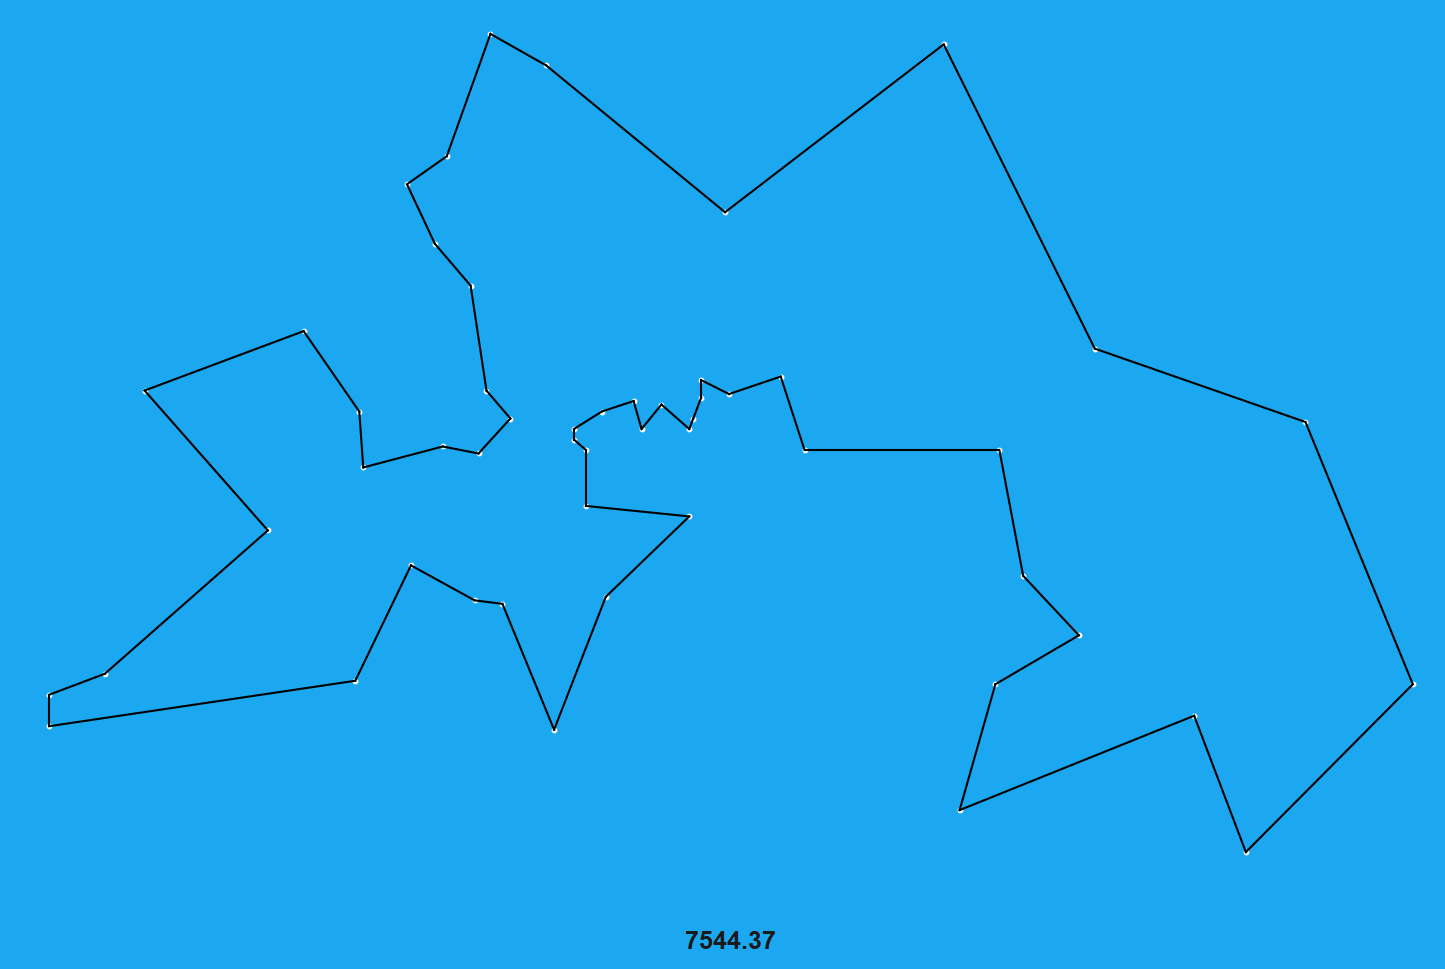
\includegraphics[width=15cm]{obrazky-figures/berlin52.png}
    \caption{berlin52}
    \label{fig:berlin52}
\end{figure}




\section{Testovací sada QA194 }
Z testovací sady s 194 místy s optimální délkou \textbf{9352} se mi nepodařilo najít optimální řešení. Pokud však na tuto sadu aplikujeme náhodné přeskupování míst před spuštěním algoritmu, dokáže ho MyAlgo poměrně rychle najít. Tuto metodu jsem však nezkoušel otestovat na větším počtu míst, protože není praktická, a chtěl jsem sjednotit testy. Nicméně MyAlgo je v porovnání s ACO lepší ve všech aspektech. ACO využívá při použití více agentů nebo jader téměř 100\% výkonu procesoru, zatímco MyAlgo nepoužívá více než 20\%. Přesto se mu podaří najít mnohem rychleji lepší řešení. Oba algoritmy využívají 2-opt algoritmus pro zlepšení řešení.


\begin{table}[H]
\centering
\caption{QA194 -- ACO}
\resizebox{\columnwidth}{!}{%
\begin{tabular}{|l|l|l|l|l|l|l|l|l|l|l|}
\hline
\textbf{Délka cesty} & \textbf{Doba běhu} & \textbf{Chybovost} & \cellcolor[HTML]{FFFFFF}{\color[HTML]{202124} \textbf{$\alpha$}} & \cellcolor[HTML]{FFFFFF}{\color[HTML]{202124} \textbf{$\beta$}} & \cellcolor[HTML]{FFFFFF}{\color[HTML]{202124} \textbf{$\rho$}} & \textbf{Q} & \textbf{Q0} & \textbf{Ag} & \textbf{It} & \textbf{C} \\ \hline
9976.41              & 7s                 & 6.6768\%           & 1                                                         & 3                                                         & 0.1                                                       & 200000     & 0.1         & 100         & 50          & 1          \\ \hline
9690.9               & 3m 20s             & 3.6238\%           & 1                                                         & 5                                                         & 0.1                                                       & 200000     & 0.1         & 300         & 150         & 6          \\ \hline
9982.26              & 1m 10s             & 6.7393\%           & 0.5                                                       & 2                                                         & 0.1                                                       & 2000       & 0.1         & 50          & 400         & 6          \\ \hline
\end{tabular}%
}
\end{table}

\begin{table}[H]
\caption{QA194 -- MyAlgo}
\centering
\resizebox{\columnwidth}{!}{%
\begin{tabular}{|l|l|l|l|l|l|l|l|l|}
\hline
\textbf{Délka cesty} & \textbf{Doba běhu} & \textbf{Bez souboru} & \textbf{Chybovost} & \textbf{SNN} & \textbf{MNN} & \textbf{LNN} & \textbf{SC} & \textbf{Segmenty} \\ \hline
9376.65              & 20s                & 15s                  & 0.2636\%           & 1            & 12           & 45           & 4           & Ano               \\ \hline
9409.45              & 6s                 & 42ms                 & 0.6143\%           & 2            & 12           & 23           & 1           & Ne                \\ \hline
9461.1               & 6s                 & 27ms                 & 1.1666\%           & 2            & 5            & 12           & 1           & Ne                \\ \hline
9509.82              & 6s                 & 205ms                & 1.6876\%           & 12           & 25           & 33           & 1           & Ne                \\ \hline
9998.15              & 6s                 & 14ms                 & 6.9092\%           & 1            & 2            & 3            & 1           & Ne                \\ \hline
9391.19              & 18s                & 13s                  & 0.4191\%           & 1            & 2            & 3            & 10          & Ano               \\ \hline
9376.65              & 1m 21s             & 1m 15s               & 0.2636\%           & 1            & 2            & 3            & 100         & Ano               \\ \hline
\end{tabular}%
}
\end{table}

\section{Testovací sada PKB411}
Jedná se o uměle vygenerovanou sadu, takže je zde velký rozdíl v zaokrouhlování vzdálenosti. Po přepočtu na desetinná čísla by  měla optimální cesta vzdálenost 1365,4. Problém je, že se to tak brát nedá, jelikož oni už ze začátku počítali s zaokrouhlenými vzdálenostmi. A optimální vzdáleností po zaokrouhlení je tedy vzdálenost \textbf{1343}. Jak zde vidíme mému algoritmu se podařilo už za 6 sekund bez optimalizací pomocí segmentů najít mnohem lepší výsledek jak ACO. Které muselo běžet 1 minutu a 17 sekund, aby našlo řešení s chybovostí skoro 7\% oproti tomu MyAlgo běžel asi 6 sekund bez překladu a generování míst je to 282ms a našel řešení s chybovostí 3.5\%. Nejlepší mnou nalezené řešení nalezl MyAlgo za 33 sekund s chybovostí zhruba 0.6\%. 

\begin{table}[H]
\caption{PKB411 -- MyAlgo bez zaokrouhlení}
\centering
\resizebox{\columnwidth}{!}{%
\begin{tabular}{|l|l|l|l|l|l|l|l|l|}
\hline
\textbf{Délka cesty} & \textbf{Doba běhu} & \textbf{Bez souboru} & \textbf{Chybovost} & \textbf{SNN} & \textbf{MNN} & \textbf{LNN} & \textbf{SC} & \textbf{Segmenty} \\ \hline
1361.08              & 32s                & 25s                  & -         & 1            & 12           & 23           & 4           & Ano               \\ \hline
1380.17              & 6s                 & 703ms                & -          & 1            & 12           & 23           & 4           & Ne                \\ \hline
1397.52              & 5s                 & 197ms                & -          & 7            & 12           & 23           & 1           & Ne                \\ \hline
1361.08              & 35s                & 29s                  & -          & 1            & 12           & 60           & 4           & Ano               \\ \hline
1367.72              & 27s                & 20s                  & -          & 1            & 5            & 5            & 1           & Ano               \\ \hline
1448.49              & 5s                 & 96ms                 & -          & 1            & 5            & 5            & 1           & Ne                \\ \hline
1628.38              & 5s                 & 19ms                 & -         & 1            & 1            & 1            & 1           & Ne                \\ \hline
\end{tabular}%
}
\end{table}

\begin{table}[H]
\centering
\caption{PKB411 -- ACO s zaokrouhlením}
\resizebox{\columnwidth}{!}{%
\begin{tabular}{|l|l|l|l|l|l|l|l|l|l|l|}
\hline
\textbf{Délka cesty} & \textbf{Doba běhu} & \textbf{Chybovost} & \textbf{$\alpha$} & \textbf{$\beta$} & \textbf{$\rho$} & \textbf{Q} & \textbf{Q0} & \textbf{Ag} & \textbf{It} & \textbf{C} \\ \hline
1499                 & 21s                & 11.6158\%          & 1         & 3         & 0.1       & 200000     & 0.1         & 100         & 50          & 1          \\ \hline
1440                 & 1m 3s              & 7.2226\%           & 1         & 13        & 0.1       & 200000     & 0.1         & 200         & 70          & 4          \\ \hline
1436                 & 1m 17s             & 6.9248\%           & 0.5       & 30        & 0.1       & 200000     & 0.1         & 200         & 140         & 4          \\ \hline
\end{tabular}%
}
\end{table}

% Please add the following required packages to your document preamble:
% \usepackage{graphicx}
\begin{table}[H]
\centering
\caption{PKB411 -- MyAlgo s s zaokrouhlením}
\resizebox{\columnwidth}{!}{%
\begin{tabular}{|l|l|l|l|l|l|l|l|l|}
\hline
Délka cesty & Doba běhu & Bez souboru & Chybovost & SNN & MNN & LNN & SC & Segmenty \\ \hline
1355        & 33s       & 26s         & 0.8935\%  & 1   & 12  & 33  & 4  & Ano      \\ \hline
1351        & 33s       & 26s         & 0.5957\%  & 5   & 12  & 23  & 1  & Ano      \\ \hline
1390        & 6s        & 282ms       & 3.4996\%  & 5   & 12  & 23  & 1  & Ne       \\ \hline
\end{tabular}%
}
\end{table}


\section{Testovací sada DJA1436}
Jedná se o uměle vygenerovanou sadu s 1436 místy. Zde budu testovat pouze testy s zaokrouhlením, jelikož je to umělá sada. Její optimální řešení má délku \textbf{5257}. Jak si můžeme všimnout mému algoritmu se oproti ACO podařilo najít rychleji mnohem kvalitnější cestu. Najít nejlepší cestu od ACO trvalo 41 minut a chybovost je poměrně velká 8,1\% oproti tomu mému algoritmu trvalo najít cestu s chybovostí pouze 3,5\% 8 sekund. 
\begin{table}[H]
\caption{DJA1436 -- ACO}
\centering
\resizebox{\columnwidth}{!}{%
\begin{tabular}{|l|l|l|l|l|l|l|l|l|l|l|}
\hline
\textbf{Délka cesty} & \textbf{Doba běhu} & \textbf{Chybovost} & \textbf{$\alpha$} & \textbf{$\beta$} & \textbf{$\rho$} & \textbf{Q} & \textbf{Q0} & \textbf{Ag} & \textbf{It} & \textbf{C} \\ \hline
5827                 & 36s                & 10.8427\%          & 1         & 3         & 0.1       & 200000     & 0.5         & 40         & 30          & 1          \\ \hline
5694                & 20m 8s              & 8.3127\%           & 1         & 13        & 0.1       & 200000     & 0.1         & 200         & 70          & 4          \\ \hline
5683                 & 41m 23s             & 8.1035\%           & 1       & 30        & 0.1       & 200000     & 0.1         & 200         & 140         & 4          \\ \hline
\end{tabular}%
}
\end{table}

\begin{table}[H]
\centering
\caption{DJA1436 -- MyAlgo}
\resizebox{\columnwidth}{!}{%
\begin{tabular}{|l|l|l|l|l|l|l|l|l|}
\hline
\textbf{Délka cesty} & \textbf{Doba běhu} & \textbf{Bez souboru} & \textbf{Chybovost} & \textbf{SNN} & \textbf{MNN} & \textbf{LNN} & \textbf{SC} & \textbf{Segmenty} \\ \hline
5366                 & 1m 41s             & 1m 35s               & 2.0734\%           & 1            & 12           & 33           & 4           & Ano               \\ \hline
5453                 & 10s                & 3s                   & 3.7284\%           & 5            & 12           & 44           & 1           & Ne                \\ \hline
5443                 & 8s                 & 1s 793ms             & 3.5381\%           & 1            & 12           & 23           & 1           & Ne          \\     \hline
\end{tabular}%
}
\end{table}




\section{Testovací sada FQM5087}

Je to uměle vygenerovaná sada s 5087 místy. Její optimální řešení má délku \textbf{13029}. Nejkratší cesta, kterou se mi povedlo za pomoci algoritmu najít má délku \textbf{13296}. Doba běhu programu trvá i s využitím segmentů maximálně do 10 minut. A nejrychlejší řešení se algoritmu povedlo najít za 35 sekund. Moje nejlepší nalezená cesta je vyobrazena na obrázku \ref{fig:FQM5087}.

\begin{table}[h]
\centering
\caption{FQM5087 -- Bez zaokrouhlení}
\resizebox{\columnwidth}{!}{%
\begin{tabular}{|l|l|l|l|l|l|l|l|l|}
\hline
\textbf{Délka cesty} & \textbf{Doba běhu} & \textbf{Bez souboru} & \textbf{Chybovost} & \textbf{SNN} & \textbf{MNN} & \textbf{LNN} & \textbf{SC} & \textbf{Segmenty} \\ \hline
13436.1              & 9m a 42s           & 8m a 27s              & -          & 1            & 12           & 23           & 4           & Ano               \\ \hline
13626.4              & 3m a 1 s           & 1m a 5s               & -          & 1            & 12           & 23           & 4           & Ne                \\ \hline
13627                & 1m a 50 s          & 35s                   & -          & 7            & 12           & 23           & 1           & Ne                \\ \hline
13429.9              & 7m a 42s           & 6m a 25s              & -           & 5            & 12           & 40           & 1           & Ano               \\ \hline
\end{tabular}%
}
\end{table}

\begin{table}[ht]
\centering
\caption{FQM5087 -- S zaokrouhlením}
\resizebox{\columnwidth}{!}{%
\begin{tabular}{|l|l|l|l|l|l|l|l|l|}
\hline
\textbf{Délka cesty} & \textbf{Doba běhu} & \textbf{Bez souboru} & \textbf{Chybovost} & \textbf{SNN} & \textbf{MNN} & \textbf{LNN} & \textbf{SC} & \textbf{Segmenty} \\ \hline
13296                & 7m 20s             & 6m 50s               & 2.0493\%           & 1            & 12           & 33           & 4           & Ano               \\ \hline
13336                & 6m                 & 5m 2s                & 2.3563\%           & 4            & 12           & 23           & 1           & Ano   \\ \hline           
\end{tabular}%
}
\end{table}


\begin{figure}[H]
    \centering
    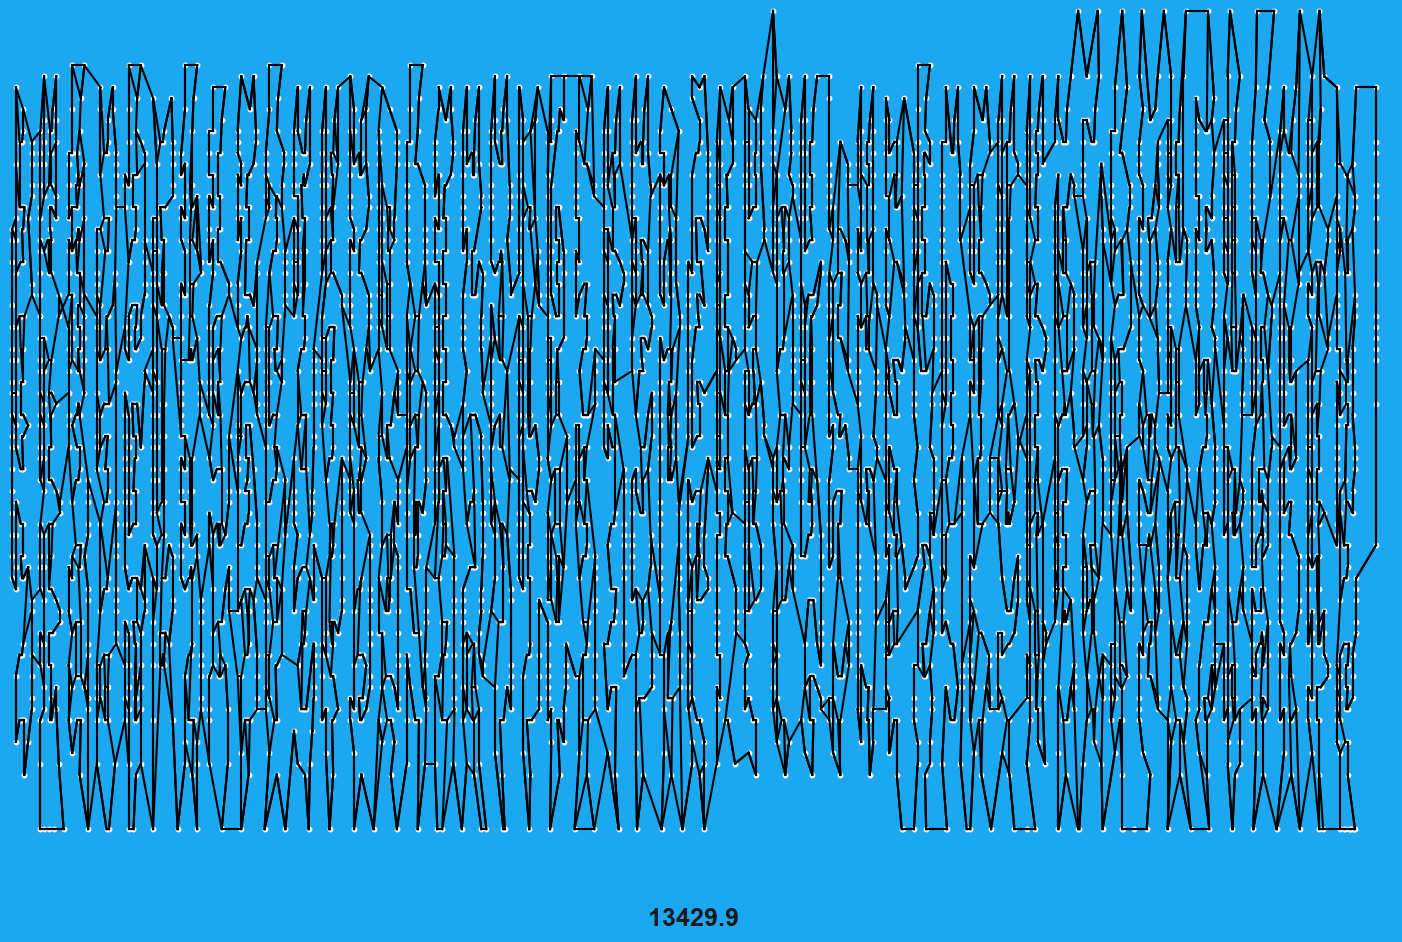
\includegraphics[width=15cm]{obrazky-figures/FQM5087.png}
    \caption{FQM5087}
    \label{fig:FQM5087}
\end{figure}

\section{Testovací sada AR9152}
Jedná se o města v státě Argentina jejich počet je 9152 a optimální cesta má délku \textbf{837479}. Mě se podařilo najít cestu dlouhou \textbf{866433}, která je vyobrazena na obrázku \ref{fig:AR9152}.

\begin{table}[H]
\centering
\caption{AR9152}
\resizebox{\columnwidth}{!}{%
\begin{tabular}{|l|l|l|l|l|l|l|l|l|}
\hline
\textbf{Délka cesty} & \textbf{Doba běhu} & \textbf{Bez souboru} & \textbf{Chybovost} & \textbf{SNN} & \textbf{MNN} & \textbf{LNN} & \textbf{SC} & \textbf{Segmenty} \\ \hline
866433               & 18m 42s            & 13m 20s              & 3.4573\%           & 5            & 12           & 23           & 1           & Ano               \\ \hline
881675               & 10m 20s            & 4m 30s               & 5.2773\%           & 5            & 12           & 23           & 1           & Ne                \\ \hline
\end{tabular}%
}
\end{table}

\begin{figure}[H]
    \centering
    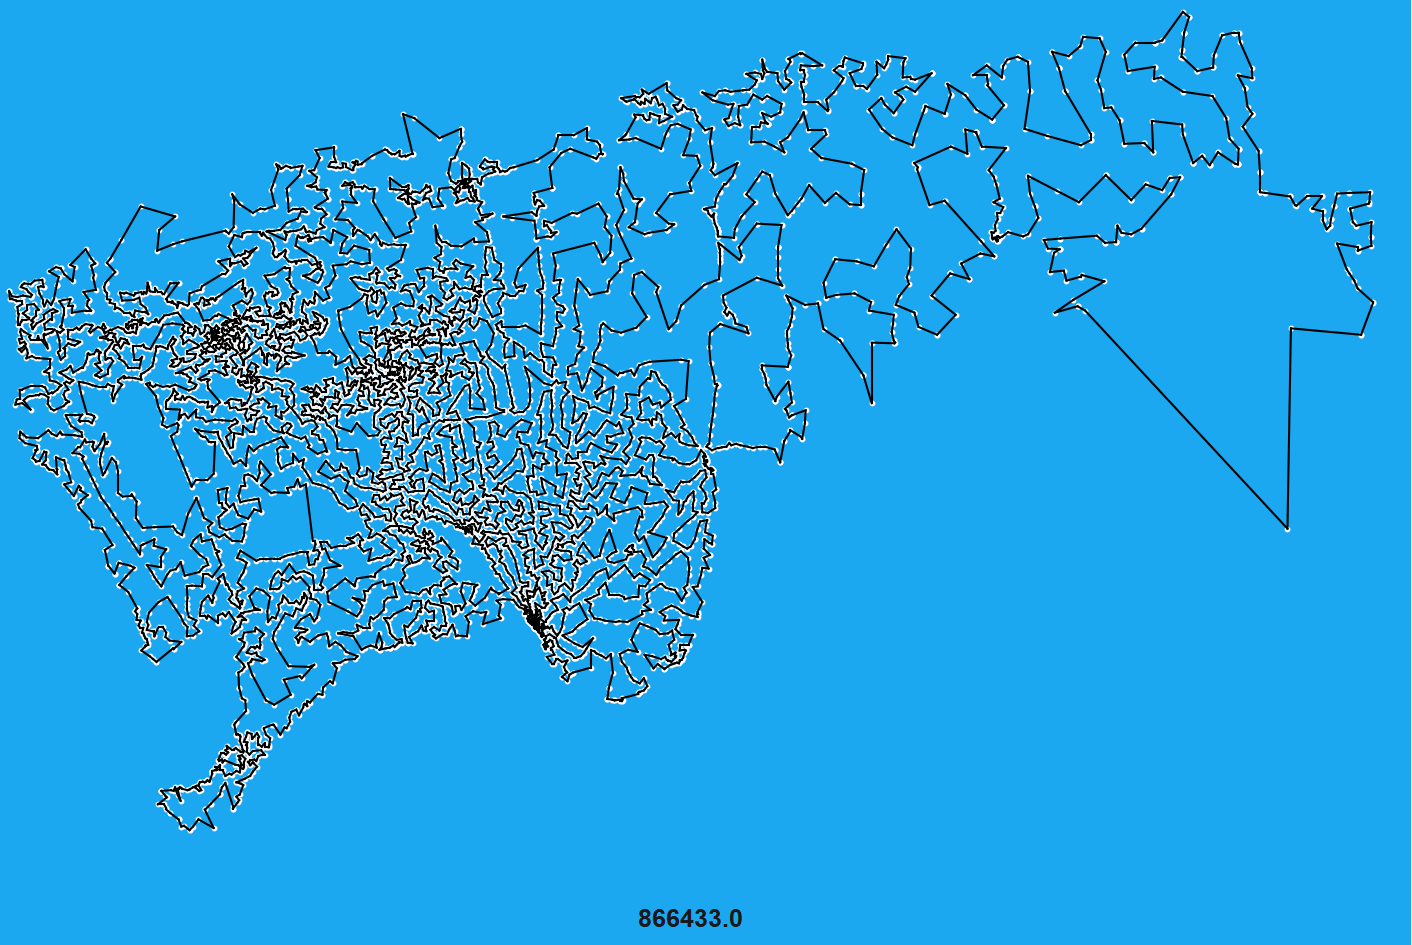
\includegraphics[width=15cm]{obrazky-figures/AR9152.png}
    \caption{AR9152}
    \label{fig:AR9152}
\end{figure}




\section{Testovací sada xmc10150}
Jedná se o uměle vygenerovanou sadu s 10150 místy. Nejlepší nalezené řešení je s délkou \textbf{28387}, které nalezl hybrid genetic algorithm od \textbf{Hung Dinh Nguyen}. Toto řešení ovšem vycházelo z již vygenerovaného řešení s délkou 28388, které nalezl \textbf{LKH} \cite{xmc10150}. Na obrázku \ref{fig:xmc10150} je zobrazeno nejlepší mnou nalezené řešení.



\begin{table}[h]
\centering
\caption{xmc10150 - Bez zaokrouhlováním}
\resizebox{\columnwidth}{!}{
\begin{tabular}{|l|l|l|l|l|l|l|l|l|}
\hline
\textbf{Délka cesty} & \textbf{Doba běhu} & \textbf{Bez souboru} & \textbf{Chybovost} & \textbf{SNN} & \textbf{MNN} & \textbf{LNN} & \textbf{SC} & \textbf{Segmenty} \\ \hline
29994.6              & 42m 5s             & 35m 3s               & -           & 1            & 12           & 33           & 4           & Ano               \\ \hline
30422.1              & 15m 6s             & 8m 24s               & -          & 7            & 12           & 23           & 1           & Ne                \\ \hline
29959.8              & 38m 2s             & 21m 12s              & -          & 1            & 12           & 40           & 1           & Ano               \\ \hline
\end{tabular}%
}
\end{table}


\begin{table}[h]
\centering
\caption{xmc10150 - S zaokrouhlováním}
\resizebox{\columnwidth}{!}{%
\begin{tabular}{|l|l|l|l|l|l|l|l|l|}
\hline
\textbf{Délka cesty} & \textbf{Doba běhu} & \textbf{Bez souboru} & \textbf{Chybovost} & \textbf{SNN} & \textbf{MNN} & \textbf{LNN} & \textbf{SC} & \textbf{Segmenty} \\ \hline
29718                & 20m 1s             & 18m 20s              & 4.6888\%           & 5            & 12           & 33           & 1           & Ano               \\ \hline
29510                & 19m                & 17m 30s              & 3.956\%            & 1            & 12           & 23           & 4           & Ano               \\ \hline
\end{tabular}%
}
\end{table}


\begin{figure}[H]
    \centering
    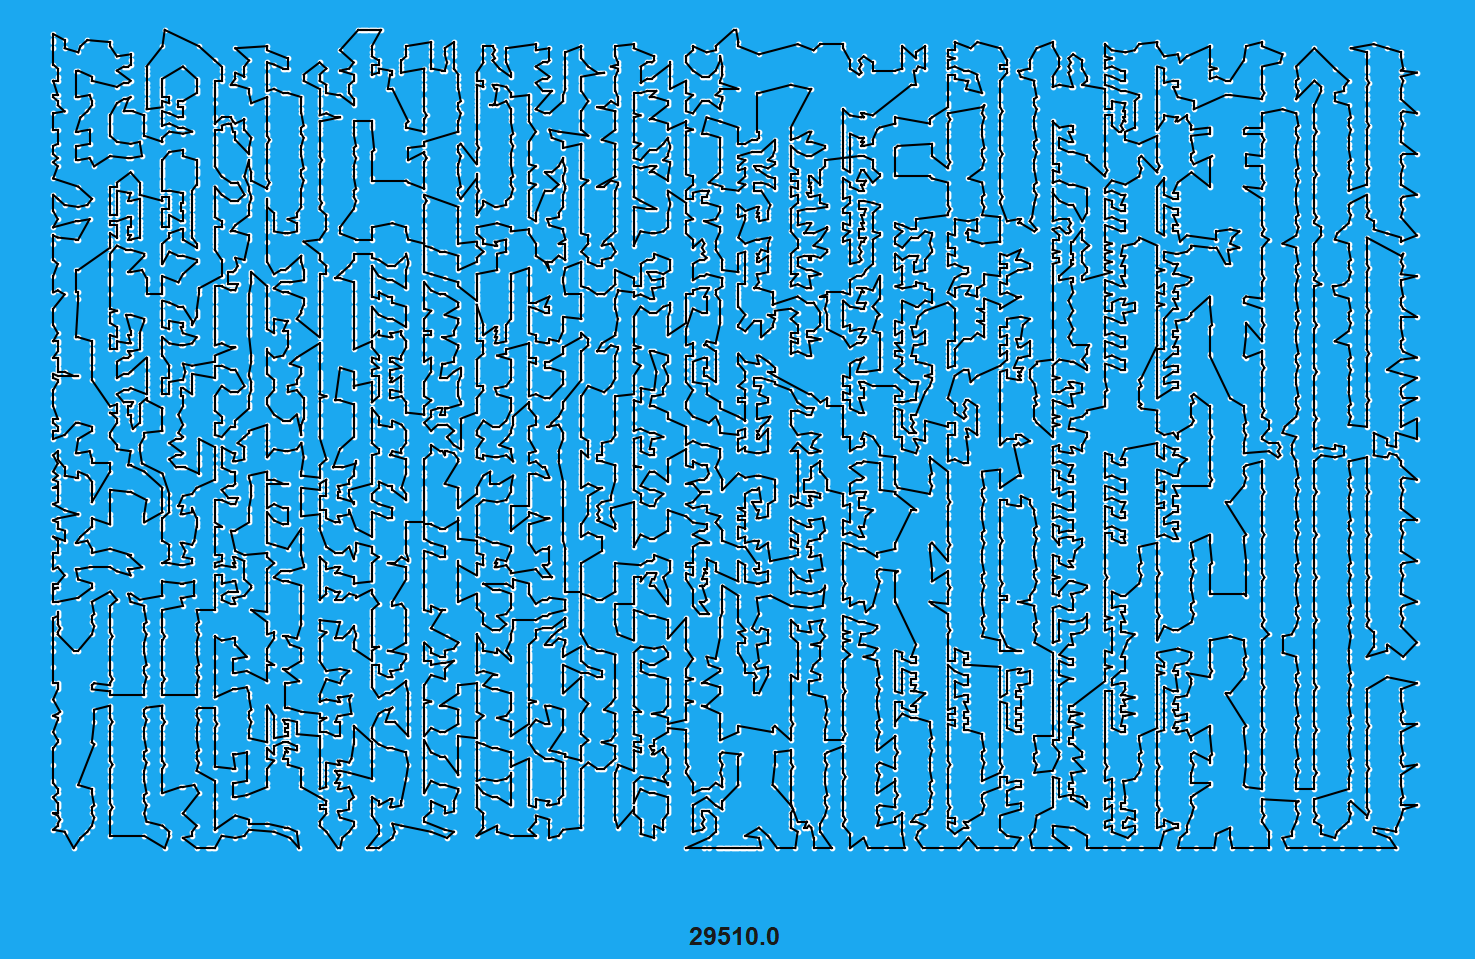
\includegraphics[width=15cm]{obrazky-figures/xmc10150.png}
    \caption{xmc10150}
    \label{fig:xmc10150}
\end{figure}

\section{Testovací sada HO14473}
Jedná se o sadu s místy v státě Honduras s 14473 místy. A nejlepší nalezenou cestou 177,092, která ovšem už vychází z předtím nalezených cest. Pro představu \textbf{LKH} běžel asi 381 hodin, aby nalezl cestu dlouhou \textbf{177,405} \cite{HO14473}. Oproti tomu MyAlgo za 16 minut nalezl řešení dlouhé 184989. A i s generováním 4 počátečních řešení mu netrvalo najít cestu dlouhou \textbf{183034} ani hodinu. Zde se začíná projevovat pomalé načítání míst do paměti, které by šlo zrychlit přidáním vláken.  Povedlo se mi neuložit si soubor s řešením s délkou 183034, tak pouze přikládám řešení s délkou 184989 zde: \ref{fig:HO14473}.



\begin{table}[H]
\caption{HO14473}
\centering
\resizebox{\columnwidth}{!}{%
\begin{tabular}{|l|l|l|l|l|l|l|l|l|}
\hline
\textbf{Délka cesty} & \textbf{Doba běhu} & \textbf{Bez souboru} & \textbf{Chybovost} & \textbf{SNN} & \textbf{MNN} & \textbf{LNN} & \textbf{SC} & \textbf{Segmenty} \\ \hline
183034               & 1h 14m             & 50m 6s               & 3.3553\%           & 1            & 12           & 33           & 4           & Ano               \\ \hline
184989               & 52m 13s            & 16m 12s              & 4.4593\%           & 1            & 12           & 23           & 1           & Ne                \\ \hline
\end{tabular}%
}
\end{table}

\begin{figure}[H]
    \centering
    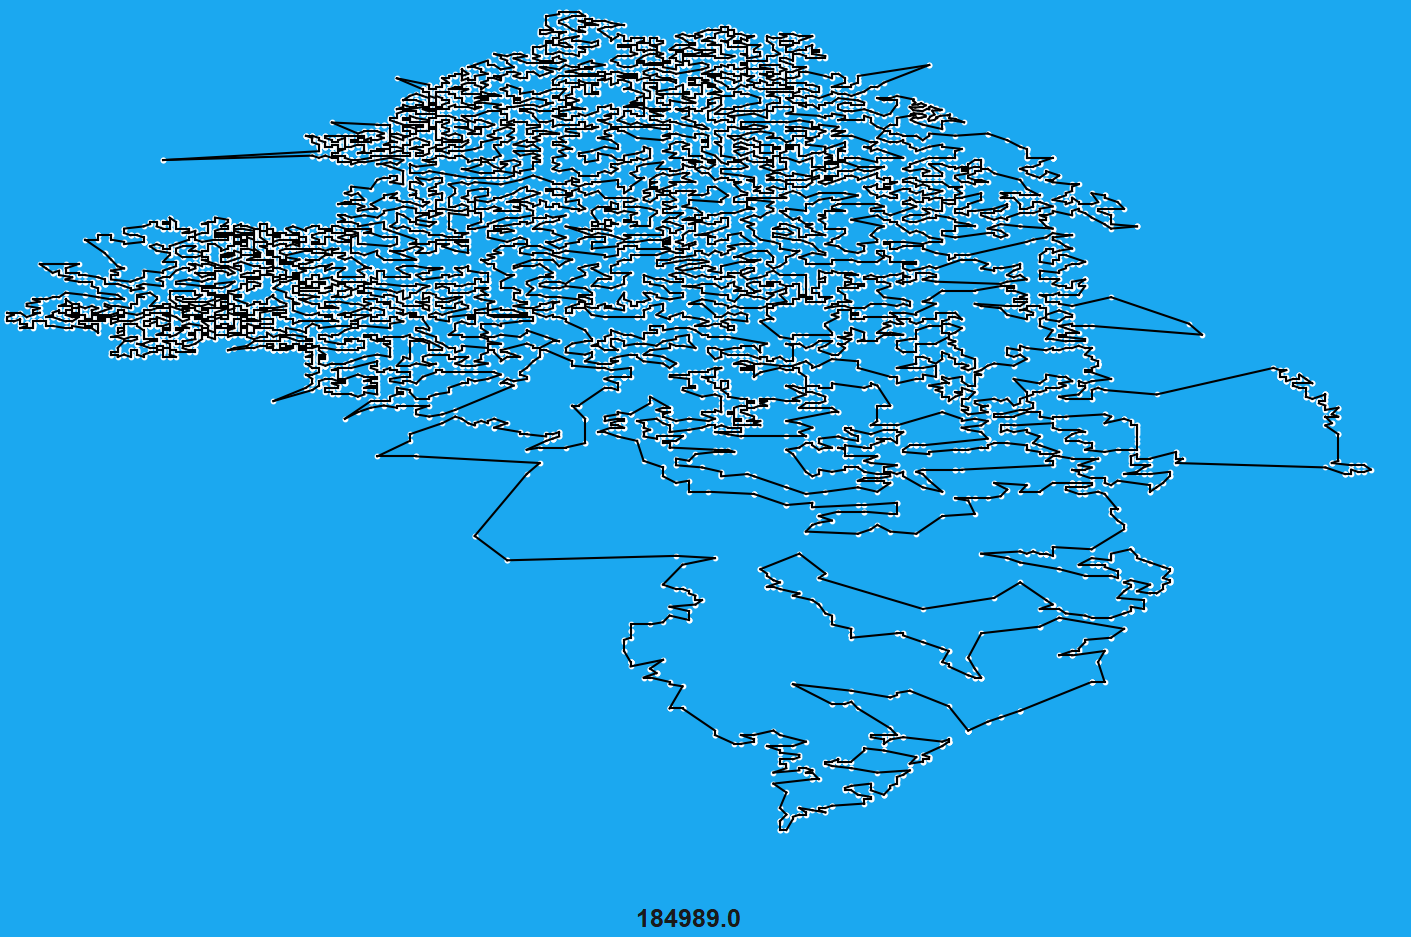
\includegraphics[width=15cm]{obrazky-figures/HO14473.png}
    \caption{HO14473}
    \label{fig:HO14473}
\end{figure}



\section{Testovací sada VM22775}
Zde se začínají projevovat hardwarové nedostatky a přesněji to, že mám k dispozici necelých 6GB operační paměti a velikost souboru s vzdálenostmi je skoro 8GB i když je rychlost algoritmu stále relativně rychlá. Program většinu času tráví v čtení a zápisu do souboru celkově 3 hodiny a 5 minut z celkové doby běhu 4 hodin a 52 minut. Je to nejspíše způsobeno tím, že operační systém musí vytvořit na pevném disku virtuální prostor pro RAM a s tím poté pracuje. Pro tuto sadu se mi povedlo najít relativně dobrý výsledek i přes to, že je zde 22775 míst. Zvýšil jsem velikost posledních sousedů a taky prvních oproti předchozím testováním. Pokud bych zde přidal víc segmentů domnívám se, že by program mohl najít řešení s chybovostí klidně okolo 1.5\%, ale prodloužil by se čas řešení. Nejlepším nalezeným řešením pro tuto sadu je \textbf{569288} a mé výsledné řešení s délkou \textbf{580836} je zde \ref{fig:VM22775}

\begin{table}[H]
\caption{VM22775}
\centering
\resizebox{\columnwidth}{!}{%
\begin{tabular}{|l|l|l|l|l|l|l|l|l|}
\hline
\textbf{Délka cesty} & \textbf{Doba běhu} & \textbf{Bez souboru} & \textbf{Chybovost} & \textbf{SNN} & \textbf{MNN} & \textbf{LNN} & \textbf{SC} & \textbf{Segmenty} \\ \hline
580836               & 4h 52m             & 1h 47m               & 2.0285\%           & 5            & 12           & 35           & 1           & Ano               \\ \hline
595972               & 4h 7m              & 1h 17m               & 4.6873\%           & 1            & 12           & 23           & 1           & Ne                \\ \hline
\end{tabular}%
}
\end{table}

\begin{figure}[H]
    \centering
    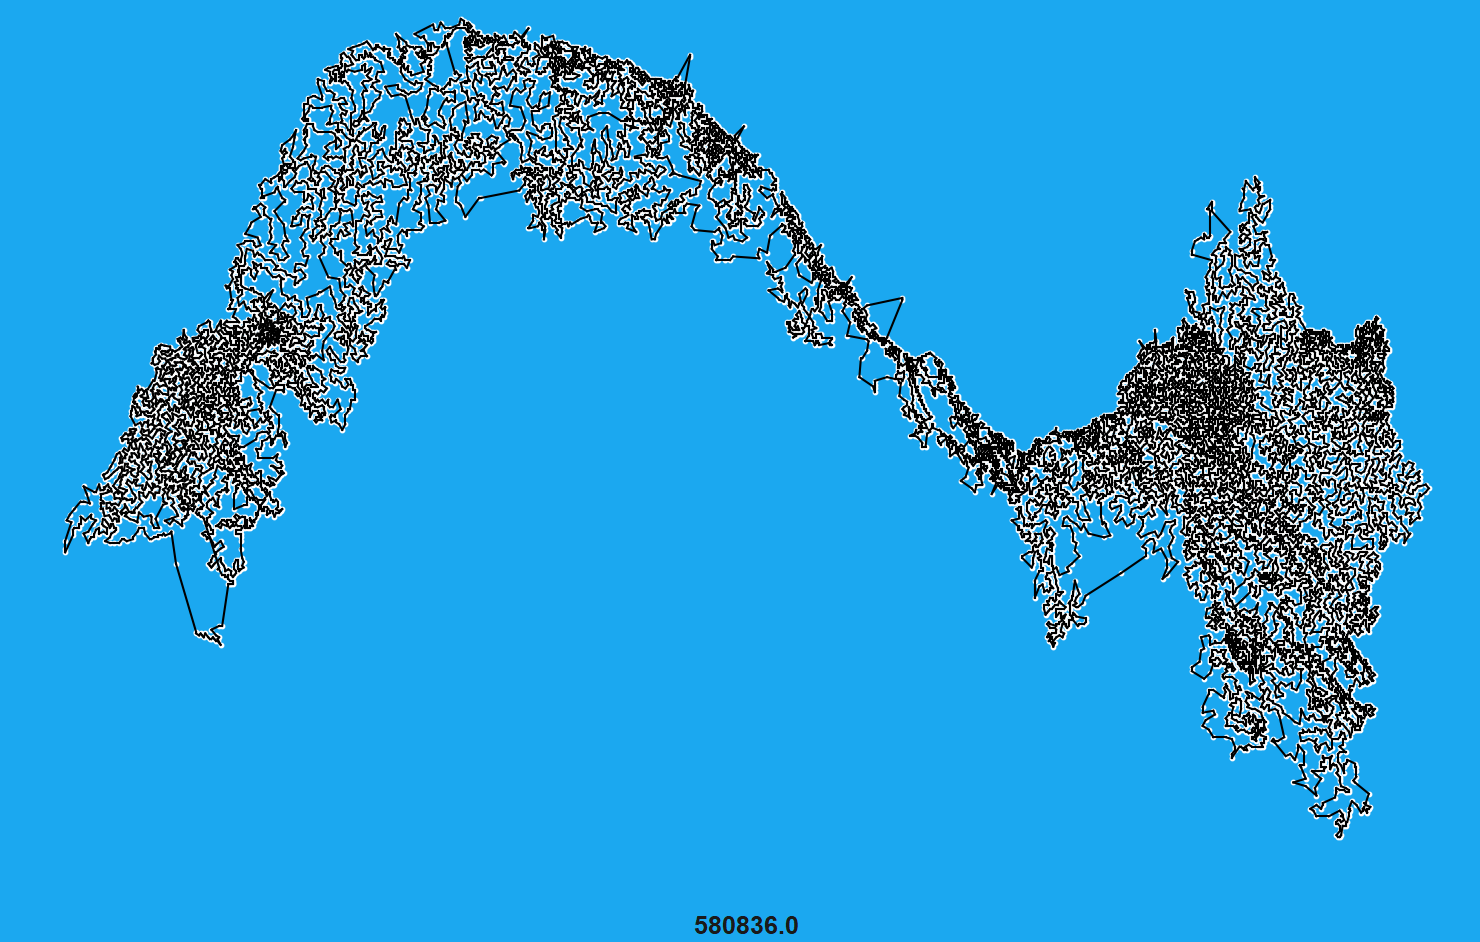
\includegraphics[width=15cm]{obrazky-figures/VM22775.png}
    \caption{VM22775}
    \label{fig:VM22775}
\end{figure}


\chapter{Návod k spuštění}
Aplikace byla vyvíjena a testována na systému 64 bitovém Windows. Ale doporučuji pro spuštění použít například Ubuntu kvůli jednoduššímu spouštění binárních souborů, jelikož ty potřebují některé dll knihovny. 
\section{Požadavky}
\subsection{Python 3.8+}
\begin{itemize}
    \item Nainstalujte Python 3.8 nebo vyšší na svůj počítač. K dispozici jsou různé zdroje, včetně oficiálního webu Pythonu (https://www.python.org/downloads/).

    \item Ověřte, zda máte nainstalovanou správnou verzi Pythonu příkazem "python --version" v příkazovém řádku nebo terminálu. Pokud je nainstalován správně, měla by se vám zobrazit verze Pythonu.
    
    \item Zkontrolujte, zda máte přístup k Pythonu z jakéhokoli adresáře v příkazovém řádku nebo terminálu. Pokud ne musíte přidat cestu k Pythonu do systémové proměnné PATH.
    \item Celkově, aby program fungoval musí fungovat příkaz "python", který spustí mezi script.
\end{itemize}
\subsection{GCC}
\begin{itemize}
\item Ověřte, zda je g++ nainstalován na vašem počítači. To můžete provést spuštěním následujícího příkazu v příkazovém řádku nebo terminálu:
\begin{verbatim}
g++ --version
\end{verbatim}

Pokud máte g++ nainstalován, zobrazí se vám informace o verzi.

\item Pokud nemáte g++ nainstalován, budete si ho muset nainstalovat. Existuje několik způsobů, jak nainstalovat g++ v závislosti na vašem operačním systému. Například pro Ubuntu a další linuxové distribuce můžete použít následující příkaz v terminálu:

\begin{verbatim}
sudo apt-get install g++
\end{verbatim}

\item Pokud jste na systému Windows program nepotřebuje překladač, stačí mu pouze, aby se ve složce System32 ve vašem počítači nacházeli potřebné dll soubory. Soubory, které se tam musí nacházet se nachází ve složce dll, k které se dostanete po rozbalení zipu. Popřípadě pokud toto nebude fungovat doporučuji nainstalovat například MinGW-w64, ale musí být k dispozici i knihovna s vlákny, které využívá ACO. 



\end{itemize}
\section{Windows}
\begin{itemize}
    
    \item Stáhněte a rozbalte zip
    \item Otevřete složku TSPSolverWindows
    \item Spustě MainWindow.exe
\end{itemize}
\section{Linux}
\begin{itemize}
    \item Stáhněte a rozbalte zip
    \item Otevřete složku 
    \item Spustě MainWindow například v termínálu pomocí ./MainWindow
\end{itemize}
\section{Ovládání programu}
Jednotlivé funkce tlačítek jsou již popsány v sekci \ref{sec:main window}. Zmíním pouze to, že pro spuštění nastavení jiného algoritmu je nutné přepnout \textbf{Algorithm types} na ten který chceme nastavit a následně stisknout tlačítko \textbf{Algorithm settings}. Algoritmus následně spustíte pomocí tlačítka \textbf{Solve}, ale předtím musí být vygenerována místa. Například, pokud jsou místa vybrána náhodně, použijte tlačítko \textbf{Generate}. Aktuální trasu smažete stiskem tlačítka \textbf{Clear roads}. Pro použití segmentů v MyAlgo je potřeba mít minimálně 130 míst, protože jsou tam pevně stanovené velikosti. Při použití \textbf{roundingu} je nutné zaškrtnout tuto volbu před generováním míst, protože v té době se počítají vzdálenosti.

\chapter{Závěr}
Cílem mé práce bylo vytvořit alespoň dva algoritmy pro řešení problému obchodního cestujícího. Hlavními algoritmy, které jsem implementoval, jsou MyAlgo a ACO. Tyto algoritmy využívají pro optimalizaci nebo například u ACO k nastavení původních feromonů i jiné algoritmy, konkrétně se jedná o Nearest Neighbor algoritmus, 3-opt a 2-opt algoritmy. Dále jsem implementoval uživatelské rozhraní pro testování a vytváření míst. U ACO se zde nachází paralelní výpočty, jak v podobě jader, tak i vláken. I přes tuto skutečnost se mi podařilo navrhnout algoritmus, který je o mnoho lepší a nepoužívá ani jádra ani vlákna. To považuji za úspěch. Jádro mého algoritmu je relativně rychlé, jelikož vždy prvně počítám vzdálenost a pokud je lepší, až poté dělám změny v poli.

Celkově si myslím, že by se dala navrhnout lepší metoda na optimalizaci mého algoritmu v podobě prohledávání více typů řešení, protože vždy existuje možnost, že aktuální řešení pomocí mého algoritmu nelze zlepšit, i když lepší řešení existuje. Nebo se zde mohla použít víc k-opt metoda pro generování například prvotních sousedů. Jenže implementace je poměrně problematická.

Metoda ACO je efektivní tak do 60 míst a dává většinou optimální výsledky v poměrně krátkém čase. Pro více než 1000 míst dává už hodně špatné výsledky s chybovostí okolo 10 \% a dobou řešení až 40 minut. Oproti tomu MyAlgo v žádné sadě nepřekonal chybovost 5 \% a i pro 22775 míst byla chybovost pouze 2 \%. Pokud srovnáme dobu běhu, ACO běží podstatně déle, proto jsem ji pro více než 1500 míst netestoval. Například k tomu, aby dosáhla chybovosti 8 \% v sadě s 1436 místy, trvalo ACO 41 minut a 23 sekund. Oproti tomu MyAlgo našel řešení s chybovostí 3.583 \% za pouhých 8 sekund a řešení s chybovostí 2 \% za 1 minutu a 35 sekund. Je možné, že pro ACO existují lepší parametry než jsem nastavil, ale po experimentování jsem lepší nastavení nenašel. V porovnání s ostatními implementacemi ACO by chybovost odpovídala.
